\documentclass[a4paper]{extarticle}
\usepackage[utf8]{inputenc}
\usepackage{hyperref}
\usepackage{geometry}
\usepackage{fancyhdr}
\usepackage{graphicx} % libreria per le immagini
\usepackage{amssymb} %libreria per i simboli (ex. alfabeto reco)
\usepackage{algorithm2e} %libreria per scrivere pseudocodice
\usepackage{longtable}
\usepackage{caption}
\usepackage{lastpage}
\usepackage{amsmath}
\usepackage{tabto}

\setlength{\parindent}{0em}%indentazione paragrafo
\setlength{\parskip}{1em}%spazio tra paragrafi
\renewcommand{\baselinestretch}{1.3}%interlinea
\graphicspath{ {./} }
\geometry{
    a4paper,
    left=10mm,
    right=10mm,
    bottom=20mm
}
\usepackage{enumitem}

\setlist{leftmargin=5.5mm}


\hypersetup{
    colorlinks=true,
    linkcolor=blue,
    filecolor=blue,      
    urlcolor=blue,
    pdftitle={Overleaf Example},
    pdfpagemode=FullScreen
}

\pagestyle{fancy}
\fancyhf{}
\rhead{Federico Calò}
\lhead{Data Mining - Appunti}
\cfoot{  \thepage }


\title{Data Mining - Appunti}
\author{\href{http://www.federicocalo.it}{Federico Calò} }
\date{}

\begin{document}
\maketitle
\newpage
\tableofcontents
\voffset -30pt

\newpage

\section{KDD process}

L'automazione delle attività economiche produce un incremento dello stream di dati perchè anche singole transazioni (una chiamata telefonica, il credito di una carta, un test medico) sono tipicamente registrate in un computer.
Le basi di dati scientifiche e governative sono in rapida crescita. C'è un divario crescente tra la generazione di dati e la loro comprensione. Risulta quindi necessario l'utilizzo di computer per analizzare i dati, ma questo non è sufficiente.

Necessitiamo di una metodologia matura che spieghi come grandi strutture di dati possono essere analizzate. Questa metodologia è stata studiata in un'area di ricerca conosciuta come KDD. Lo scopo è investigare come tecniche di Machine Learning possono essere applicate a estratti di "conoscenza" di una grande massa di dati disponibili. All'inizio vi era una certa confusione sull'area di interesse ricoperta dal Machine learning, Data Mining e Knowledge Discovery. Ora, si è giunti alla conclusione che il KDD denota l'intero processo di estrazione della conoscenza, dalla raccolta dei dati per poi effettuare una pre-elaborazione degli stessi fino  all'interpretazione dei risultati.

Il Data Mining è lo step, all'interno del processo KDD, nel quale le informazioni sono estratte dai dati applicando ad essi opportuni algoritmi. Questi algoritmi sono il più delle volte quelli di Machine Learning. 
In un contesto aziendale il termine Data Mining è ancora utilizzato per denotare il processo di knowledge discovery e questo causa qualche confusione. Sempre sulla terminologia: KDD è ancora utilizzato anche se la conoscenza non è rigorosamente estratta dai "database". 

Si potrebbe definire il Knowledge Discovery come un processo nell seguente modo: "Il Knowledge Discovery è l'estrazione non banale di informazioni implicite, precedentemente sconosciute e potenzialmente utili dai dati."
\begin{itemize}
    \item \textbf{Non banale}: si intende che nel processo è coinvolta qualche ricerca o inferenza statistica, quindi non è un semplice calcolo di quantità predefinite;
    \item \textbf{Implicita}: ci si riferisce al fatto che l'informazione è implicita nel dato e non formalmente esplicita, l'informazione esplicita è estratta attraverso altre tecniche;
    \item \textbf{Sconosciuta}: l'informazione deve essere nuova, la novità dipende dal quadro di riferimento assunto;
    \item \textbf{Utile}: l'informazione deve essere utile a raggiungere lo scopo del sistema o dell'utente. I pattern completamente estranei agli obiettivi dati sono di scarsa utilità e non costituiscono conoscenza all'interno della situazione data.
\end{itemize}

Possiamo formalmente definire il KDD nel seguente modo:

\textbf{Dati}:
\begin{itemize}
	\item un insieme di fatti (data) F,
	\item una rappresentazione in un linguaggio L,
	\item una certa misura di certezza C,
\end{itemize}
possiamo definire un pattern come una dichiarazione S in L che descrive le relazioni tra un sotto insieme $F_{S}$ di F con una certezza \textbf{\textit{c}}, tale che S è più semplice (in un certo senso) dell'enumerazione di tutti i fatti in $F_S$.

Un pattern è considerato conoscenza se è interessante e abbastanza certo (o valido). Nel KDD siamo interessati in pattern che sono espressi in un linguaggio di alto livello, come:
\newpage
\begin{center}
Se Età $<$ 25 e Corso-di-Educazione = no

Allora Incidente = si

Con probabilità = 0.2 a 0.3
\end{center}
In questo modo alcuni pattern possono essere capiti e usati direttamente dalle persone o possono essere input ad altri programmatori.
Definiamo ora il termine \textbf{certezza} come qul livello sufficiente di certezza senza il quale i modelli diventano ingiustificati e non riescono a diventare conoscenza. La certezza coinvolge diversi fattori, quali: 
\begin{itemize}
	\item Integrità dei dati;
	\item Dimensione del campione su cui è stata effettuata la scoperta;
	\item Il grado di supporto dalla conoscenza del dominio disponibile.
\end{itemize}

Un pattern è definito \textbf{interessante} quando è:
\begin{itemize}
	\item Nuovo;
	\item Utile;
	\item Non banale da calcolare.
\end{itemize}

Vi sono principalmente due differenti interpretazioni dei pattern e dei modelli.
La \textit{prima interpretazione} che possiamo dare consiste nel definire un \textbf{modello} come una sintesi globale del data-set, mentre il \textbf{pattern} è una caratteristica locale del data-set, limitato a un sub-set di osservazioni e/o attributi.
La \textit{seconda interpretazione} esplica come il data mining implica l'adattamento o la determinazione di pattern da dati osservati. In questo caso il pattern è visto come una istanza del modello. I modelli adattati svolgono il ruolo di conoscenza dedotta.

Il KDD è un processo iterativo e interattivo, costituito da molti passaggi che includono molte decisione prese dall'utente.

\begin{figure}[h]
\noindent
\makebox[\textwidth]{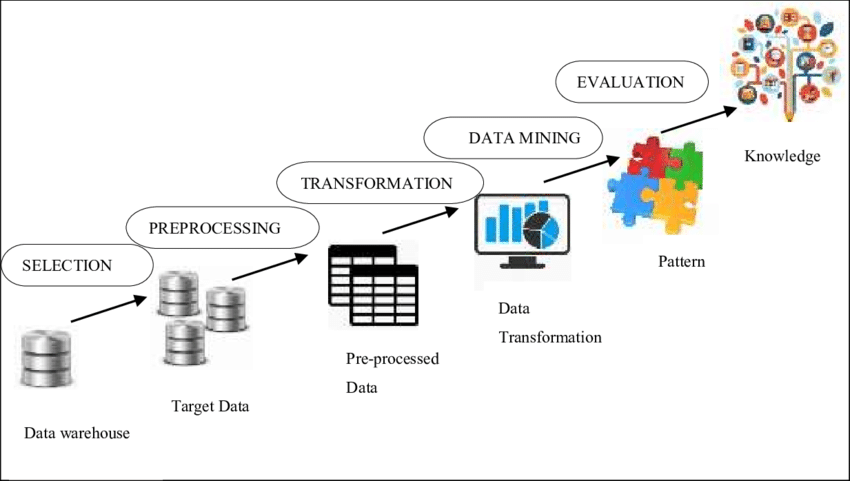
\includegraphics[width=12cm]{kdd-process}}%
\end{figure}

In una prima fase si sviluppa una \textbf{comprensione del dominio} dell'applicazione, delle relative conoscenze di base e degli obiettivi dell'utente finale. Si prosegue creando \textbf{un data set target}, selezionando un dataset o ci si focalizza su un sotto insieme di variabili o di esempi di dati sui quali deve essere eseguita la scoperta. Una volta selezionati questi dati si passa alla fase di \textbf{pulizia dei dati e preprocessing} nella quale si effettuano svariate operazioni volte a rimuovere il rumore o dei valori anomali, collezionando le informazioni necessarie per modellarle o tenere conto del rumore, decidere strategie per gestire i campi di dati mancanti o tenere conto delle informazioni sulla sequenza temporale e delle modifiche note. Successivamente si entra in una fase di \textbf{riduzione e proiezione dei dati}, nella quale si trovano funzioni utili per rappresentare i dati a seconda dell'obiettivo dell'attività. Vengono utilizzati metodi di riduzione o trasformazione multidimensionale per ridurre l'effettivo numero di variabili da considerare o per trovare rappresentazioni di dati invarianti. Conclusa questa attività, si passa alla \textbf{selezione del task di data mining}, decidendo qual è l'obiettivo del processo KDD, scegliendo tra classificazione, regressione, clustering. 

Definito l'obiettivo si passa alla \textbf{scelta degli algoritmi} di data mining. Vengono selezionati i metodi che verranno utilizzati per ricercare i pattern frequenti all'interno dei dati. Vengono definiti i modelli e i parametri più appropriati e si cerca di far corrispondere particolari metodi di data mining con i criteri globali dei processi di KDD. Quindi si entra nella fase di \textbf{Data Mining}, nella quale si ricercano modelli di interesse in una particolare forma rappresentativa.  L'utente può contribuire significativamente in questa fase eseguendo correttamente i passaggi precedenti. Alla fine del processo di data mining, vi è la fase di \textbf{interpretazione dei pattern minati}, nella quale si effettuano le valutazioni sui risultati ottenuti ed eventualmente si ritorna ad iterare su uno degli step precedenti. Infine si \textbf{consolida la conoscenza scoperta}, incorporando la conoscenza ottenuta nel sistema per migliorarne le prestazioni o semplicemente si documenta per essere segnalata ad altre parti di interesse. Questa fase include anche il controllo e la risoluzione di particolar conflitti con conoscenze precedentemente estratte o scoperte.

\subsection{Steps del KDD}

La maggior parte del lavoro nel KDD è focalizzata sullo step del data mining. Anche se gli altri step sono considerati importanti per il successo dell'applicazione del KDD nella pratica. La necessità per una standardizzazione del processo della scoperta della conoscenza ha portato alla definizione dello standard industriale CRISP-DM. L'obiettivo di questo standard è quello di sviluppare un processo neutrale per condurre il KD,  e di definire i compiti, i loro outputs, la terminologia e i problemi tipici di caratterizzazione. 

Il modello di processo CRISP-DM è per la scoperta i conoscenza consiste in sei fasi.

\begin{center}

\fbox{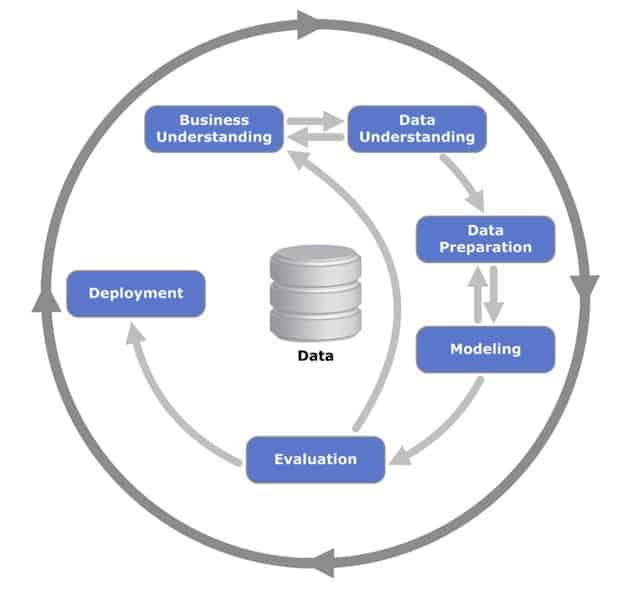
\includegraphics[width=.4\textwidth, height=.3\textheight, keepaspectratio]{crisp-dm-model}}

\end{center}

La sequenza delle fasi non è rigida. È possibile spostarsi avanti e indietro tra le diverse fasi a seconda dell'esito di ciascuna fase. Le frecce indicano le dipendenze più importanti/frequenti. Il cerchio esterno simboleggia la natura ciclica di un processo KDD che può continuare dopo l'implementazione di una soluzione. Ogni fase contiene un numero di task che produce specifici output.

\subsubsection{Business Understanding}

La \textit{prima fase} di questo modello viene definita \textbf{Business Understanding}, il cui primo step è quello di determinare gli obiettivi commerciali. I requisiti minimi sono:

\begin{itemize}
	\item un problema o un'opportunità commerciale percepita
	\item un certo livello di sponsorizzazione esecutiva
\end{itemize}

Sviluppare una definizione chiara e comprensibile dei bisogni aziendali non è un compito semplice. E' richiesta la collaborazione dei \underline{business analyst} e dei \underline{data analyst}. Questo passaggio del processo è anche il momento in cui iniziare a definire le aspettative. Alla fine di questo step vengono prodotti:

\begin{itemize}
	\item \textbf{Il background}, che descrive le informazioni note sulla situazione aziendale all'inizio del processo;
	\item \textbf{Gli obiettivi di business}, che descrivono i principali obiettivi dal punto di vista del business;
	\item \textbf{I criteri economici di successo}, che definiscono le misure per risultati di alta qualità del progetto dal punto di vista del business.
\end{itemize}

Dopo aver definito gli obiettivi commerciali, si passa alla \textbf{valutazione della situazione}, con lo scopo di raccogliere informazioni sulle risorse, sui vincoli e sulle assunzioni. Alla fine di questo sotto processo verrà prodotto un inventario contenente:

\begin{itemize}
\item le risorse: personale, dati, calcoli;
\item vincoli: schede di compilazione, questioni legali, comprensibilità;
\item assunzioni: disponibilità dei dati;
\end{itemize}

Inoltre non dimentichiamo che vengono prodotti anche \textbf{un glossario di termini}, che copre la terminologia di business e di data mining, e \textbf{un'analisi costo-beneficio}, cioè un documento contenente le spese del progetto dovrebbero essere confrontate con i potenziali guadagni.

Successivamente si passa alla \textbf{determinazione degli obiettivi del Data Mining}. In questa fase si trasformano gli obiettivi commerciali in obietti del processo di Data Mining e si costruiscono i relativi criteri di successo. Possiamo classificare gli obiettivi del Data Mining in:

\begin{itemize}
\item Classification
\item Estimation (produrre una stima, Estimation)
\item Prediction
\item Affinity grouping
\item Clustering
\item Description e Profiling
\end{itemize}

I due obiettivi primari del Data Mining tendono ad essere:

\begin{itemize}
\item \textbf{Predizione}, che include l'uso di alcune variabili indipendenti per predire valori sconosciuti o futuri che dipendono da altre variabili;
\item \textbf{Descrizione}, nella quale non si fa una distinzione tra variabili dipendenti e indipendenti e si concentra sulla ricerca di modelli interpretabili dall'uomo che descrivono i dati.
\end{itemize}

L'obiettivo della classificazione è apprendere una funzione che mappa, o classifica, un dato in una predefinita classe. Questa tecnica è molto utilizzata per i database. Invece quando si parla di regressione, si ha come obiettivo apprendere una funzione che mappa un dato in una variabile di previsione reale. Quando  si cerca di creare un procedimento per trovare le associazioni tra gruppi di variabili, si utilizza il metodo Affinity Grouping. Il clustering è un'attività descrittiva in cui si cerca di identificare un insieme finito di categorie o cluster per descrivere i dati. Le categorie possono essere mutuamente esclusive ed esaustive, oppure consistere in una rappresentazione più ricca come una gerarchia o categorie sovrapposte. La clasterizzazione viene utilizzata spesso per scoprire sotto-popolazioni omogenee, identificare sotto categorie, o analisi di dati. Strettamente correlato al clustering è il compito della stima della densità di probabilità, che consiste in tecniche per stimare dai dati la funzione di densità di probabilità multivariata congiunta di tutte le variabili/campi nel database.
Per \textbf{Summarization} (riassunto o descrizione o profilazione), si intendono tutti quei metodi per trovare una descrizione compatta per un sottoinsieme di dati. Invece il task \textbf{Dependency modeling} (modellare le dipendenze), consiste nel trovare un modello che descrive dipendenze significative tra variabili. Esistono due tipi di modelli dipendenti:
\begin{itemize}
\item il livello strutturale di specifici modelli le cui variabili sono localmente dipendenti tra loro
\item il livello quantitativo il cui modello specifica quanto le variabili sono dipendenti usando una scala numerica.
\end{itemize}
Il task di rilevamento di modifiche e deviazioni si focalizza sulla scoperta delle modifiche più significanti nei dati rispetto a valori misurati o normativi in precedenza. Consiste nel trovare un modello che descrive significanti dipendenze tra variabili.

Dopo aver definito il task del Data Mining si passa a \textbf{produrre un piano progettuale} per il raggiungimento egli obiettivi di data mining e quindi il raggiungimento degli obiettivi di business. L'output di questa fase è ovviante un piano progettuale, che specifica l'insieme degli step per la restante parte del progetto, la sua durata, le risorse richieste, gli input, gli output e le dipendenze.

\subsubsection{Data Understanding}

Dopo aver contestualizzato il business in cui si andrà a progettare il sistema, si passa a una fase di \textbf{Data Understanding}, cioè di compresone dei dati, che inizia con una fase di raccolta iniziale dei dati. Durante questa fase si accede ai dati rilevanti nell'inventario delle risorse e si produce un report iniziale dei dati raccolti, nel quale si elenca la posizione dei dati, i metodi usati per acquisirli e i problemi incontrati. Successivamente si passa a descrivere i dati esaminando le loro proprietà e creando un report nel quale si descrive il formato dei dati, i potenziali valori, la quantità, l'identificatore dei campi e tutte le caratteristiche che vengono scoperte.

Ci sono due metodi principali per descrivere le variabili:

\begin{itemize}
\item \textbf{variabili categorighe}: i possibili valori finiti e i differenti tipi che una variabile può assumere. Questa categoria si può suddividere in:
	\begin{itemize}
	\item \textbf{variabili nominali} che denominano il tipo di oggetto a cui si riferiscono, ma non esiste un 	ordine tra i valori possibili. (stato del materiale, genere, livello di educazione)
	\item \textbf{variabili ordinali} che assumono un ordine tra i possibili valori. (valutazione del cliente)
	\end{itemize}

\item \textbf{variabili quantitative}: sui quali sono consentite operazioni aritmetiche, e si suddividono a loro volta in:

\begin{itemize}
	\item \textbf{variabili discrete}, i cui valori sono interi
	\item \textbf{variabili continue}, i cui valori sono numeri reali.
	\end{itemize}

\end{itemize}

Dopo aver descritto la tipologia di dati si passa alla verifica della loro qualità ispezionando e affrontando diverse caratteristiche quali:

\begin{itemize}
\item \textbf{Accuratezza}: conformità del valore memorizzato rispetto a quello effettivo
\item \textbf{Completezza}: nessun valore mancante
\item \textbf{Consistenza}: rappresentazione uniforme
\item \textbf{Attualità}: i dati storicizzati non sono obsoleti.
\end{itemize}

\textit{Scarsa qualità dei dati} e \textit{scarsa integrità dei dati} sono i maggiori problemi all'interno dei progetti KDD. La maggior parte dei dati operativi non è mai stata acquisita o modellata per scopi di data mining. I dati selezionati vengono generalmente raccolti da numerosi sistemi operativi, incoerenti e scarsamente documentati. È importante comprendere la \textbf{sensibilità temporale} dei dati. Lo specialista della gestione dei dati è responsabile della raccolta e dell'integrazione dei dati nell'ambiente informativo. 

Al termine della verifica della qualità dei dati viene gerato un report di qualità dei dati che riporta i risultati della verifica e se vi sono dei problemi, sarà possibile discutere di eventuali soluzioni.

A valle della verifica della qualità dei dati, è possibile avviare la fase di \textbf{esplorazione dei dati}, alla fine della quale seguirà un relativo report dei risultati ottenuti. Per le \textit{variabili categoriche}, le distribuzioni della frequenza dei dati sono il metodo migliore per capire il contenuto dei dati. Istogrammi e grafici a torta aiutano a identificare gli schemi della distribuzione e i valori mancanti o non validi. Mentre quando lavoriamo con \textit{variabili quantitative}, l'analista dei dati è interessato a misure come il massimo e il minimo, la media, moda, mediana e misure statistiche. Se combinate, queste misure offrono un modo efficace per determinare la presenza di dati non validi e distorti.

\subsubsection{Data Preparation}

Lo step successivo al Data Understang vi è lo step di \textbf{Data Preparation}, la cui prima fase consiste nel selezionare i dati, nella quale il problema maggiore consiste nel selezionare dati da tuple di database relazionali. Si possono comunque seguire alcuni principi che includono:
\begin{itemize}
\item la rilevanza del dato rispetto all'obiettivo principale.
\item vincoli tecnici e qualitativi,
\item limiti al volume dei dati o ai tipi di dati
\end{itemize}

In questa fase si produce un report di inclusione/esclusione dei dati. La selezione dei dati può essere eseguita manualmente o automaticamente (campionamento e selezione delle caratteristiche).

Il più semplice tipo di campionamento è il \textbf{Simple random sampling} (campionamento semplice casuale): ogni gruppo di oggetti della dimensione richiesta ha la stessa probabilità di essere il campione selezionato. È possibile ottenere un campione molto atipico, tuttavia le leggi della probabilità impongono che più ampio è un campione, più è probabile che sia rappresentativo della popolazione da cui proviene. 

Il metodo tradizionale di scelta di un campione casuale inizia con una numerazione dei membri della popolazione target. L'ordine di numerazione è irrilevante. Una volta che ogni membro della popolazione ha un numero, il campionatore consulta una tabella di numeri casuali per selezionare gli indici dei membri da includere nel campione. Ovviamente il presupposto principale è quello di essere in grado di numerare i membri della popolazione target. 

Vi sono due tipi di campionamento semplice casuale:
\begin{itemize}
\item con sostituzione
\item senza sostituzione
\end{itemize}

Se la popolazione è grande rispetto al campione, c'è una probabilità molto piccola che qualsiasi membro venga scelto più di una volta e le due tecniche sono essenzialmente le stesse.

Quando la popolazione è divisa in strati o gruppi, è utile invece usare un \textbf{campionamento casuale stratificato}. Viene selezionato un campione casule semplice da ciascuno strato separatamente e la loro unione produce un campione stratificato. Un vantaggio di questo campionamento consiste nel fatto che l'analista può controllare il numero di osservazioni all'interno di ogni gruppo o strato e può garantire che particolari gruppi all'interno della popolazione sono adeguatamente rappresentati nel campione. Quando uno strato ha un'appartenenza molto più piccola degli altri, il semplice campionamento casuale può produrre campioni senza rappresentativi di quello strato. La dimensione del campione è solitamente proporzionale alla dimensione relativa degli strati. Tuttavia, questa non è una regola.

Se i membri all'interno degli strati sono più simili tra loro rispetto ai membri di strati diversi, le stime specifiche per strato saranno più precise di quelle dell'intero campione. Attenzione però, è importante adeguarsi alla sovra rappresentazione quando le inferenze si riferiscono alla popolazione target nel suo insieme.

Alcune regole per una buona rappresentazione di progettazione per un campionamento stratificato, sono:
\begin{itemize}
\item gli strati devono essere scelti per:
	\begin{itemize}
	\item avere dei mezzi che differiscono sostanzialmente tra loro
	\item minimizzare la varianza all'interno di uno strato e massimizzarla tra i vari strati
	\end{itemize}
\item Le dimensioni del campione devono essere proporzionali alla deviazione standard dello strato.
\end{itemize}

Un'altra tecnica di campionamento è il \textbf{cluster sampling} o campionamento clusterizzato, nel quale i membri della popolazione arrivano naturalmente da cluster, ciò rende possibile campionare i cluster. In questo caso tutti i membri di ogni cluster sono considerati. Nel contesto di grandi basi di dati, un'applicazione comune del cluster sampling è di rendere casuale la scelta di blocchi di dati, e successivamente usare tutti i dati nei blocchi. La motivazione dietro questo approccio è che per recuperare un record di database da un blocco particolare, l'intero blocco deve essere letto in memoria. Questo tipo di campionamento è anche chiamato \textbf{block scampling}. I vantaggi del cluster sampling riguardano la riduzione dei costi richiesti per accedere ai campioni, e al tempo stesso aumenta la variabilità delle stime campionarie al di sopra di quella del semplice campionamento casuale, a seconda di quanto i cluster differiscono tra loro, rispetto alla variazione all'interno del cluster.

Se i membri di un cluster sono più simili dei membri di cluster diversi, gli approcci statistici che presuppongono che i dati siano indipendenti porteranno a inferenze distorte. La modellazione gerarchica può modellare esplicitamente la struttura indotta dall'amplificazione nei dati.

Il \textbf{two-stage sampling} (campionamento a due stadi) combina due idee principali: la celta casuale dei cluster e il campionamento all'interno di ogni cluster. 

Quando è possibile numerare in qualsiasi modo gli individui di una popolazione, si può effettuare il \textbf{systematic sampling} (campionamento sistematico), conosciuto anche come \textbf{every k-th sampling}. Questo tipo di campionamento si sviluppa scegliendo un membro in maniera casuale da quelli numerati tra 1 e k, successivamente include ogni k-th membro dopo il campione.  Il vantaggio maggiore di questo tipo di campionamento è la sua facile implementazione,anche nel caso in cui la dimensione della popolazione è inizialmente sconosciuta o il conteggio dei membri della popolazione è computazionalmente costoso. Al contempo bisogna prestare attenzione, dato che la selezione non è casuale, campioni sistematici possono non essere rappresentativi della popolazione e quindi devono essere utilizzati con attenzione. Questo metodo è particolarmente vulnerabile alle periodicità nell'elenco dei membri della popolazione. Se la periodicità è presente e il periodo è un multiplo di k, risulterà una distorsione.

Quando vogliamo organizzare il nostro campionamento basato sul valore di una o pù variabili, ma non conosciamo l'intervallo o la distribuzione di queste variabili nella popolazione target, possiamo avvalerci del \textbf{two-phase sampling} o campionamento in due fasi. Un campione iniziale può facilitare prendere decisioni più consapevoli sulle strategie di campionamento da utilizzare.
Un campione iniziale può aiutare a determinare la dimensione del campione. I calcoli delle dimensioni del campione spesso richiedono stime di determinati parametri della popolazione, come la forza della relazione tra due variabili. In assenza di conoscenze e/o dati pregressi, un campione iniziale fornirebbe stime per queste quantità e queste stime determinerebbero la dimensione del campione per il campione della seconda fase.

Una domanda che ci si pone spesso è quanto un campione deve essere grande. In statistica vi sono semplici meccanismi per stimare la dimensione del campione necessaria per avere una certa probabilità di rilevare un effetto di una dimensione pre-specificata o superiore. Questi meccanismi, che raggruppati prendono il nome di \textit{analisi di potenza}, si basano su stime delle medie e varianze delle variabili nella popolazione da campionare. E' importante capire il sistema di cause che determinano popolazione e garantire che tutte le fonti di variazione siano prese in considerazione. Un gran numero di osservazioni non ha alcun valore se le principali fonti di variazione vengono trascurate nello studio.

Un'alternativa ad impostare una dimensione del campione predeterminata consiste nel lasciare che i dati "scelgano" la dimensione del campione. L'idea di base è continuare ad aumentare la dimensione del campione fino a quando i risultati o i riepiloghi non cambiano più molto (dove "molto" è impostato in anticipo). Le varianti di questa idea sono note come campionamento progressivo, campionamento adattivo o campionamento sequenziale.

Bisogna però far attenzione al fatto che molti degli strumenti comuni per l'inferenza statistica, inclusi i t-test, presuppongono che i dati comprendano un semplice campione casuale di una popolazione e che i singoli punti dati siano quindi statisticamente indipendenti. Molte delle tecniche di campionamento violeranno questa ipotesi. Esistono tecniche statistiche specializzate per trattare i dati generati da un numero qualsiasi di  campionamento casuale da un database fornisce stime imparziali delle caratteristiche del database. Tuttavia, se il database stesso rappresenta un campione casuale o sistematicamente distorto dalla popolazione reale di interesse, nessuna tecnica statistica può salvare le inferenze risultanti.

I database in tempo reale contengono degli attributi (chiamati anche \textbf{features} o caratteristiche). Il problema della selezione delle caratteristiche sorge perchè la complessità di ricerca nello spazio delle ipotesi deve essere ridotta per ragioni pratiche, e caratteristiche ridondanti o irrilevanti possono avere effetti significativi sulla qualità dei risultati del metodo di analisi (\textbf{maledizione della dimensionalità}). L'idea alla base della maledizione della dimensionalità è che dati di grande dimensione sono difficili da processare, per una serie di motivi: il numero di esempi cresce esponenzialmente con il numero di variabili e non ci sono abbastanza osservazioni per ottenere buone stime.

La \textbf{feature selection} è un processo che scegli un subset ottimo di features seguendo alcuni criteri. Vi sono sostanzialmente 3 approcci:
\begin{itemize}
\item \textbf{wrapper models}
\item \textbf{filter models}
\item \textbf{embedded methods}
\end{itemize}

Il \textit{wrapper model} si basa su un algoritmo di data mining per determinare se un sottoinsieme di funzionalità è valido. L'algoritmo viene utilizzato come parte della funzione di valutazione e anche per indurre i patterns o il modello finale. 

L'algoritmo DM può risolvere task predittivi o task descrittivi. Se vogliamo avere un buon insieme di funzionalità per migliorare l'accuratezza di un classificatore, possiamo utilizzare proprio questa misura per basare le evoluzioni del classificatore. Però sorgono diversi problemi, il principale consiste nel determinare veramente l'accuratezza predittiva evitando l'overfitting. Altri problemi consistono nel fatto che un classificatore richiede tempo per apprendere i dati, oppure i dati sono troppo grandi per eseguire un algoritmo di apprendimento, quindi è necessario ridurne la dimensionalità. Vi è quindi la necessità di definire alcuni criteri di stop per garantire che il processo di valutazione termini e che non entri in un loop infinito.

Il filter models è indipendente dall'algoritmo di data mining che sarà utilizzato sul subset di feature. I subset sono valutati utilizzando proprietà intrinseche dei dati quali le misure informative e di distanza. Se consideriamo l'accuratezza stimata da un classificatore come un'altra misura, possiamo unificare i modelli di filtering e wrapper in un modello generale. Ogni componente può avere diverse scelte. Le varie combinazioni di queste scelte sono alla base di molti algoritmi di selezione delle caratteristiche esistenti.

Alcune strategie per la selezione delle caratteristiche dei subset sono:
\begin{itemize}
\item \textbf{enumerazione} di tutte i possibili subset e selezione dei migliori
\item \textbf{generazione casuale} dei subset e selezione del migliore.
\item \textbf{generazione sequenziale} dei subsets.
\end{itemize}

Possiamo inoltre selezionare i subset attraverso la \textbf{foward selection}, iniziando con un subset vuoto e gradualmente aggiungere una caratteristica alla volta, oppure attraverso lla \textbf{backward selection}, nel quale si inizia con un insieme completo e si rimuove una caratteristica alla volta. Queste strategie sono basate sulla \textbf{strategia di ricerca greedy} in uno spazio di subset grande $2^N$, dove N è il numero di caratteristiche.

Indipendentemente dal metodo di generazione dei sottoinsiemi di funzionalità adottato, è necessaria una misura per decidere quale funzionalità deve essere aggiunta o rimossa, oppure quale sottoinsieme deve essere mantenuto. Questo è possibile grazie alla \textbf{misura dell'informazione}, data una funzione di incertezza \textbf{U} e le probabilità delle classi precedenti \textbf{P($c_i$)}, l'informazione ottenuta da una caratteristica X, \textbf{IG(X)}, è definita come la differenza tra la precedente incertezza e l'incertezza posteriore attesa usando X. In formula
\begin{equation}
IG(X)= \sum_{i} U(P(c_i))-E[\sum_{i}U(P(c_i|X))
\end{equation}

Una regola di valutazione delle caratteristiche derivata dal concetto di guadagno di informazioni afferma che la caratteristica X è preferita alla caratteristica Y se $IG(X)>IG(Y)$. Cioè, una caratteristica dovrebbe essere selezionata se può ridurre più incertezza. Se U(x)=$-x*log(x)$ allora $\sum_{i}U(P(c_i))$ è una misura di entropia.

\textbf{\textit{Misure della distanza.}} Se l'obiettivo è la classificazione, una misura alternativa può essere la distanza tra le funzioni di densità classe-condizione. Se \textit{P($X|C$)} è la funzione di densità condizionata dalla classe della caratteristica X, nei due casi della clase (C=$c_1$ o C=$c_2$),P($X|C$) è definita da P($X|c_1$) e P($X|c_2$). Se D(X) è la distanza tra P($X|c_1$) e P($X|c_2$), una regola di valutazione basata su P afferma che X è preferito a Y se D(X)$>$D(Y). Questo perchè stiamo cercando una feature che può separare due classi il più possibile. Maggiore è la distanza, più facile separare le due classi.

La \underline{divergenza Kullback-Leibler} è una misura della distanza tra distribuzioni probabili, P e Q su un dominio V. Questa divergnza è definita come:

\begin{equation}
m_{KL}(P,Q)= \sum_{v\in V} q(v)log(\dfrac {q(v)}{p(v)})
\end{equation}

Questa divergenza misura in quale misura la distribuzione P è un'approssimazione della distribuzione Q o, più precisamente, la perdita dell'informazione se noi prendessimo P invece di Q. In sintesi si misura quanto P diverge da Q. LE proprietà di questa misura sono:

\begin{itemize}
\item Assimetrica, ovvero $m_{KL}(P,Q) \not = m_{KL}(Q,P)$
\item non definita quando p(v)=0
\item nel caso specifico di q(v)=0, q(v)log(q(v)/p(v))=0
\item il range dei valori non è limitato. Quindi, possiamo utilizzare questo valore per stabilire quale delle due distribuzioni Q e Q' è una migliore approssimazione di P, ma non ci permette di determinare in termini assoluti se Q è una buona approssimazione di P osservando $m_{KL}(P,Q)$
\end{itemize} 

La divergenza del $\chi ^2$ è definita come:

\begin{equation}
m \chi ^2(P,Q) = \sum_{y \in Y} \dfrac{|p(y)-q(y)|^2}{p(y)}
\end{equation}

è rigorosamente topologicamente più forte della divergenza KL data la disuguaglianza $m_{KL}(P,Q) \leq m \chi ^2 (P,Q)$, la convergenza nella funzione di divergenza $\chi ^2$ implica la convergenza nella divergenza KL, ma non il contrario. Inoltre è assimetrica e non definita quando p(y)=0.

Un ultimo tipo di misura della distanza eè la distanza di variazione, data dalla formula $m_1 (P,Q)= \sum_{y \in Y}|p(y)-q(y)|$, detta anche distanza di Manhattan per funzioni di probabilità p(y) e q(y) e coincide con la distanza di Hamming quando tutte le features sono binari. Similarmente si può utilizzare la distanza Euclidea data da $m_2 (P,Q)= \sum_{y \in Y} |p(y)-q(y)|^2$. Queste due metriche soddisfano la proprietà di simmetria e le proprietà metriche.

\textbf{\textit{Dipendenza dalle misure}}. Si verifica con quanta forza una caratteristica è associata alla classe. Denotando attraverso R(X) una misura di dipendenza tra la feature X e la classe C, preferiamo la feature X alla feature Y se R(X)$>$R(Y). Un problema con le tre misure precedenti è che non possono rompere i legami tra due features ugualmente buone. Pertanto queste funzionalità non possono rilevare se una di esse è ridondante.

\textbf{\textit{Inconsistenza delle misure}}. Si tenta di trovare un numero minimo di funzionalità che separano le classi in modo coerente come può fare l'intero set di funzionalità. In altre parole, le misure di incoerenza mirano a raggiungere $P(C|FullSet)= P(C|SubSet)$ Le regole di valutazione delle funzionalità derivate dalle misure di incoerenza affermano che è necessario selezionare il sottoinsieme minimo di funzionalità in grado di mantenere la coerenza dei dati mantenuti dall'insieme completo di funzionalità.

Per \textbf{selezionare le feature} ci sono 3 componenti necessari: un generatore di subset, un valutatore e un criterio di stop. Vi sono diversi metodi. 

\textbf{\textit{Approcci completi ed esaustivi}}: il \textit{focus} è applicato su una misura di consistenza e valuta esaustivamente tutti i subset partendo da una feature, mentre il \textit{branch and bound} consiste in una enumerazione sistematica di tutte le soluzioni, dove ampi sottoinsiemi di candidati infruttuosi sono scartati in massa utilizzando dei limiti superiori e inferiori della quantità da ottimizzare. Inizia con un insieme completo di feature e valuta l'accuratezza stimata. 

\textbf{\textit{Approcci Euristici}}: \textbf{\textit{SFS}} (sequential foward search) e \textbf{\textit{SBS}}(sequential backward search) possono essere applicati a ciascuna delle misure, \textbf{\textit{DTM}} è la più semplice versione  di una modalità di weapper - impara un classificatore una volta e usa qualsiasi caratteristica trovata nel classificatore. 

\textbf{\textit{Approcci non deterministici}}: \textbf{\textit{LVF}} (Las Vegas Filter) e \textbf{\textit{LVW}} (Las Vegas wrapper), generano subset di feature casualmente e li testano in maniera differente, LVF applica una misura inconsistente, LVW usa una stima accurata attraverso un classificatore; \textbf{\textit{algoritmi generici}} e \textbf{\textit{ricottura simulata}} sono anche usati nella selezione di feature. Il primo può produrre più sottoinsiemi, il secondo produce un singolo sottoinsieme.

\textbf{\textit{Approcci basati sulle instanze}}: \textbf{\textit{Relief}}, molti piccoli campioni di dati sono campioni proveniente dai dati. Le funzionalità vengono ponderate in base ai loro ruoli nella differenziazione di istanze di classi diverse per un campione di dati. È possibile selezionare funzioni con pesi maggiori. 

Per le attività di data mining non di classificazione (nessuna etichetta di classe disponibile), dovrebbero essere presi in considerazione metodi alternativi. Ad esempio, una misura di entropia può essere introdotta per classificare in sequenza le caratteristiche. L'idea di base è che le caratteristiche sono rilevanti se possono descrivere le istanze in termini di cluster relativamente chiaramente definiti.

La \textbf{scalabilità} è un altro problema. In LVS la parte più dispendiosa in termini di tempo di un processo di selezione delle funzionalità viene identificata e ritardata fino a quando non è necessario. LVS è un'estensione di LVF che utilizza una misura di incoerenza (IC) con una complessità di runtime di controllo O(n), dove n è il numero di istanze. Se n è enorme, è costoso calcolare IC molte volte. Si noti inoltre che il componente di generazione di sottoinsiemi di funzionalità genererà sempre più sottoinsiemi non validi che non soddisfano IC man mano che la cardinalità di un sottoinsieme valido diminuisce. 

Pertanto, ha senso separare il calcolo di IC come cardinalità per tutti i dati dalla generazione di sottoinsiemi di funzionalità. Ma abbiamo bisogno di dati per generare sottoinsiemi di funzionalità. Il compromesso è che invece di utilizzare l'intero set di dati, ne utilizziamo solo una parte per la generazione di sottoinsiemi di funzionalità. Quando un sottoinsieme viene testato come valido sulla porzione di dati, viene calcolato l'IC per l'intero dato. Successivamente se IC è stato soddisfatto, allora la selezione della feature è completata, altrimenti se IC non è stato soddisfatto, le istanze inconsistenti vengono aggiunte alla porzione di dati e viene eseguito un altro ciclo di generazione di sottoinsiemi di funzionalità sulla porzione di dati ingrandita. Questo metodo è particolarmente efficace solo quando n è sufficientemente largo a causa del sovraccarico nel LVS.

I \textbf{wrapper models} cercano di risolvere uno specifico problema, quindi il criterio può realmente essere specificato. Invece consuma molto tempo se bisogna valutare uno schema a ogni iterata. I \textbf{filter models} sono molto più veloci  ma non incorporano algoritmi di data mining usati per la generazione di un modello o pattern, quindi il modello può essere subottimale.

A differenza dei precedenti, nei \textbf{metodi embedded} la parte di selezione delle caratteristiche non può essere separata dall'algoritmo di data mining. È parte integrante dell'algoritmo. Per esempio, nell'algoritmo di decision tree, la selezioni delle caratteristiche che contribuiscono alla creazione dell'albero finale è parte della costruzione dell'algoritmo di decision tree. Poiché siamo interessati a selezionare le funzionalità nella fase di trasformazione dei dati, non consideriamo gli embedded methods.

La \textbf{pulizia dei dati} aumenta la qualità dei dati al livello richiesto. Ciò comporta la selezione di sottoinsiemi di dati puliti, l'inserimento di impostazioni predefinite adeguate o tecniche più ambiziose come la stima della modellazione dei dati mancanti. Alla fine di questa fase vi è un rapporto sulla pulizia dei dati, che descrive le decisioni e le azioni per affrontare i problemi di qualità dei dati ed elenca le trasformazioni dei dati per la pulizia e i possibili impatti sull'analisi dei risultati. I due problemi più comuni sono la mancanza di valori e dati di rumore. 

I \textbf{noisy data}, ovvero tutti quei dati che generano rumore, consistono in variabili che hanno valori non conformi con quelli che ci aspettiamo dalle variabili. Le osservazioni in cui si verificano questi noisy data sono chiamate valori anomali, ovvero (\textit{outliers}). Differenti tipi di outliers possono essere trattati in differenti modi. 

Vi possono essere errori umani, i quali possono essere corretti o cancellati dall'analisi, oppure le distribuzioni simmetriche spesso indicano valori anomali. La mancanza di dati, invece, include valori che non sono presenti nei dati selezionati e necessitano di essere eliminati durante il rilevamento del rumore. Questo caso si verifica se viene commesso un errore durante l'inserimento dei dati, oppure se l'informazione non era disponibile al momento dell'inserimento oppure se i dati selezionati all'interno di risorse eterogenee hanno creato dei mismatch. 

Per correggere questo tipo di errore vengono eseguite diversi tipi di azioni, l'inserimento di un valore predefinito come il termine "none" è l'ideale. Si potrebbe cancellare le righe che presentano valori mancanti, però questa tecnica, per quanto facile da implementare, può generare la perdita di dati che possono essere valutati. 

Un'altra tecnica consiste nell'eliminazione della variabile dall'analisi se presnta un significativo numero di osservazioni con valori mancanti per la stessa variabile. Infine, un'ultima tecnica, consiste nel rimpiazzare il valore mancante con un altro valore, che nel caso di variabili quantitative può consistere nella media o nella mediana, mentre per le variabili categoriche può essere rappresentato dalla moda o dal valore "sconosciuto". Si potrebbe anche pensare di attuare un approccio più sofisticato è quello di predire il valore più probabile delle variabili all'interno delle osservazioni.

Successivamente si passa alla fase di \textbf{costruzione dei dati}, la quale include operazioni di preparazione dei dati, come la generazione di variabili derivate, inserimento di nuovi record o trasformazione di variabili esistenti. I dati possono essere trasformati in \textit{una singola variabile}, per essere ulteriormente perfezionati per soddisfare i requisiti del formato di input dei particolari algoritmi di data mining da utilizzare.

Esempi sono la conversione delle variabili di tipo data dal formato US a quello Europeo, oppure il calcolo dell'età data la data di nascita, l'aggregazione dei valori all'interno di un conto corrente per gli ultimi 3,6,12 mesi. Inoltre si potrebbe effettuare un ridimensionamento o una normalizzazione dei dati. In questo caso si parla di normalizzazione dei dati quando colonne numeriche sono trasformate usando funzioni matematiche in dei range. Questo processo è importante perchè tutte le variabili all'interno di una colonna devono essere trattate in maniera uguale e non devono influenzarsi a vicenda, oppure perchè alcuni dati possono ricevere solo alcuni valori all'interno di un range.

Un altro tipo di normalizzazione è la normalizzazione min-max che performa una transformazione lineare sui dati originali. Supponendo che $ min_A$ e $max_A$ sono i valori di minimo e di massimo di un attributo A, questa normalizzazione mappa un valore v di A in v' nel range $[newMin_A; newMax_A]$ attraverso la formula:
\begin{equation}
v'= \dfrac{v-min_A}{max_A-min_A}(newMax_A - newMin_A)+newMin_A
\end{equation}

Le relazioni tra i valori dei dati originali vengono preservate. Se un caso di input futuro per la normalizzazione non rientra nell'intervallo di dati originale per A, si verifica un errore "out of bounds" (fuori dal limite).

Nella normalizzazione definita z-score, anche chiamata a media zero, i valori per un attributo A sono normalizzati sulla base della media o della deviazione standard di A. Un valore v di A è normalizzato in v' attraverso la formula:

\begin{equation}
v'=\dfrac{v-mean_A}{standDev_A}
\end{equation}

dove $mean_A$ e $standDev_A$ sono la media e la deviazione standard dell'attributo A. Questo metodo di normalizzazione è utile quando il minmo e il massimo dell'attributo A sono sconosciuti, o quando ci sono gli outliers che dominano la normalizzazione min-max.

La normalizzazione attraverso il decimal scaling transforma i valori dell'attributo A in punti decimali, per assicurarsi che il range dell'intervallo i cui essi sono compresi sia \{-1,+1\}. Il numero di punti decimali dipende dal massimo valore assoluto di A. Un valore v di A è normalizzato in v' attraverso la funzione:

\begin{equation}
v'= \dfrac{v}{10^j}
\end{equation}

dove j è il più piccolo intero tale che $max(|v'|)<1$

Si parla di \textbf{discretizzazione delle variabili} quando convertiamo variabili quantitative in variabili categoriche dividendo il valore di input in intervalli. Due metodi di discretizzazione sono l'\textbf{Equale Width} e l'\textbf{Equal depth}. In entrambi questi metodi le informazioni sulla classe non vengono utilizzate nel caso in cui le osservazioni siano preclassificate, inoltre la discretizzazione viene applica a ogni attributo indipendentemente dagli altri. 

Il partizionamento attraverso l'equal width divide il range in N intervalli di uguale lunghezza, se A e B sono il più piccolo e il più grande valore all'interno dell'attributo, l'intervallo di width sarà:

\begin{equation}
W=\dfrac{B-A}{N}
\end{equation}

Questo metodo è il più diretto, però ha anche degli aspetti negativi perchè non gestisce bene i dati distorti ed è sensibile ai valori anomali.

Il partizionamento attraverso l'equal-depth divide il range in N intervalli, ognuno contenente approssimativamente lo stesso numero di esempi. Questo tipo di partizionamento ha una buona scalabilità, gestisce gli attributi categorici attraverso alcuni trucchetti, minimizza le informazioni perdute durante il processo di partizionamento.

In entrambi i casi il numero di elementi tralasciati è definito dall'utente. Nel caso di classificazione dei dati, è buona pratica che questo numero non sia minore del numero di classi che vogliamo riconoscere, oppure determinarlo attraverso la formula:

\begin{equation}
N_{bins} = \dfrac{M}{3*C}
\end{equation}

dove M è il numero di esempi di training e C il numero di classi.

Procedure complesse di conversione di dati hanno l'obiettivo di costruire un piccolo insieme di indici da un vasto numero di variabili, in modo tale che solo alcune informazioni vengano perse e il numero totale di funzioni venga ridotto. \textbf{L'analisi fattoriale} e \textbf{l'analisi del componente principale} sono due tecniche di analisi multivariate per la riduzione dei dati. 

\textit{L'analisi fattoriale} affronta il problema dell'analisi della struttura delle interrelazioni (correlazioni) tra un grande numero di variabili (ad es. punteggi dei test, elementi del test, risposte al questionario) definendo un insieme di dimensioni sottostanti comuni, note come fattori. Questa non è una tecnica che usa dipendenze, ovvero non vi è nessuna variabile considerata come criterio o variabile dipendente da cui tutte le altre dipendono e sono le variabili predittore o indipendenti. E' una tecnica interdipendente in cui ogni variabile è considerata simultaneamente e ognuna è in relazione alle altre.

Oltre alla costruzione dei dati, vi è l'integrazione dei dati, che ha come obiettivo la combinazione di informazioni provenienti da tabelle multiple o record per creare nuovi record o valori. L'output di questa fase è un insieme di dati uniti, che si riferisce all'unione di due o più tabelle unite che contengono differenti informazioni sugli stessi oggetti, o dati aggregati, sui quali verranno effettuate delle operazioni per produrre nuovi dati. Il risultato è il modello dei dati analitici, che rappresenta una ristrutturazione consolidata, integrata e dipendente dal tempo dei dati selezionati e pre-elaborati dalle varie fonti operative ed esterne. 

Una decisione importante presa in questo compito riguarda l'unità di analisi. Nella ricerca nelle scienze sociali, le unità di analisi più tipiche sono le persone individuali. Altre unità di analisi possono essere gruppi, manufatti (libri, foto, giornali), unità geografiche (città, censimento, stato), interazioni sociali (relazioni diadiche, divorzi, arresti). L'unità di analisi non deve essere confusa con le unità di osservazione, che è l'unità su cui vengono raccolti i dati, cioè vengono effettuate osservazioni sistematiche. Ad esempio, uno studio può avere un'unità di osservazione a livello individuale (ad es. alunni), ma può avere l'unità di analisi a livello di gruppo (ad es. una classe). L'unità di osservazione è la stessa dell'unità di analisi quando le generalizzazioni ricavate da un'analisi statistica sono attribuite all'unità di osservazione (cioè gli oggetti su cui i dati sono stati raccolti e organizzati per l'analisi statistica).

Un'altra procedura consiste nel formattare la sintassi di alcuni tipi, non andando ad alterare i significati, perchè questi formati sono richiesti da altri modelli.

\subsubsection{Modeling}

In questa fase viene scelta la tecnica di modellazione tra le tecniche e gli strumenti preselezionati, come output si hanno le tecnice e le assunzioni modellate dalle tecniche prese in input. Ci sono diversi fattori su cui basare la scelta dell'algoritmo o degli algoritmi per modellare i dati, tra cui la natura dell'obiettivo, la capacità di gestire determinati tipi di dati, la capacità di gestire multiple relazioni e generare pattern relazionali, la scalabilità o il livello di famigliarità. 

Si possono identificare tre componenti primari in qualsiasi algoritmo di data mining:
\begin{itemize}
\item \textbf{modello di rappresentazione}: relazionale o proposizionale, qualitativo o quantitativo, adeguatezza per un utente.
\item \textbf{modello di valutazione}: l'incertezza del modello si base su stime probabilistiche, test statistici ecc.
\item \textbf{ricerca}
\end{itemize}

Il \textit{modello di rappresentazione} consiste nel linguaggio L usato per descrivere patterns che possono essere scoperti. Dipende dal tipo di rappresentazione, la capacità descrittiva, l'adeguatezza per un dato utente. La conoscenza scoperta può essere categorizzata dal tipo di pattern dei dati. Una scoperta quantitativa mette in relazione valori di campi numerici usando equazioni matematiche, mentre una relazione qualitativa mette in relazione logica diversi campi. Spesso si possono trovare queste due relazioni combinate. Un altro aspetto che bisogna considerare nella creazione del modello è la sua rappresentazione che deve essere appropriata per l'utente previsto. 

La maggior parte degli utenti per i quali bisogna creare una rappresentazione sono gli umani, programmi per computer e sistemi di scoperta. Se si parla di utenti umani bisogna utilizzare un linguaggio naturale, molto utile ma non conveniente per la manipolazione da parte di algoritmi di scoperta, oppure si potrebbe utilizzare un linguaggio logico, molto più utile per la computazione e se necessario può essere anche traslato in un linguaggio normale. Le informazioni sulla forma e la densità dei gruppi di record sono un altro tipo di conoscenza che si presenta al meglio visivamente per mezzo di grafici bidimensionali o tridimesionali, quindi attraverso opportune rappresentazioni visive. 

Nel caso in cui gli utenti finali siano dei programmi, la rappresentazione include linguaggi di programmazione e formalismi dichiarativi. Quando invece l'utente è un sistema il cui compito è scoprire conoscenza, le nuove scoperte vengono reinserite nel sistema come conoscenza di dominio, la conoscenza di dominio e la conoscenza scoperta devono condividere una rappresentazione comune. Se la rappresentazione è limitata, nessun addestramento o nessun tipo di esempio produrrà un modello accurato per i dati. È importante che un analista di dati comprenda appieno i presupposti rappresentativi che possono essere inerenti a un particolare metodo.

Alcuni patterns sono spesso associati a un grado di incertezza, rappresentata attraverso la probabilità, la deviazione standard, misure di credenza o fuzzy sets. In maniera visiva l'informazione incerta può essere convertita in dimensione, densità e ombreggiatura.

Quando i database sono veramente grandi, con milioni di record, un'analisi completa di tutti i dati è infattibile. Gli algoritmi di rilevamento devono quindi basarsi su una qualche forma di campionamento, per cui viene considerata una parte dei dati. Le scoperte risultanti in questi casi sono necessariamente incerte. Le tecniche statistiche possono misurare il grado di incertezza. Possono anche essere utilizzati per determinare la quantità di campionamento aggiuntivo necessaria per ottenere il livello di fiducia desiderato nei risultati.

Il modello di valutazione stima l'incertezza di un particolare pattern. Ci sono diversi metodi per valutare questa incertezza. La \textbf{cross validation} è una di queste procedure che consiste nel mescolare i dati del dataset, partizionarli in k sottoinsiemi di uguale lunghezza n, per ogni sottoinsieme chiama i-esimo subset di n oggetti come insieme test e lo mette da parte, addestra il sistema sui rimanenti sottoinsiemi e testa il sistema sull'insieme di test e memorizza le performances,  successivamente pulisce la memoria dimenticando ciò che ha imparato durate l'addestramento, calcola le performance medi di ogni insieme di test.

La scelta dell'algoritmo di data mining è fondamentale per conoscere se la ricerca dovrebbe essere performata nello spazio dei parametri o nello spazio dei modelli o entrambi. Se non è possibile una soluzione, si possono utilizzare metodi iterativi greedy. 

La ricerca del modello avviene come un ciclo sul metodo di ricerca dei parametri, la cui rappresentazione viene modificata in modo da considerare una famiglia di modelli. Per ogni rappresentazione specifica del modello viene istanziata la modalità di ricerca dei parametri per valutare la qualità di quel particolare modello. Le implementazioni dei metodi di ricerca del modello tendono a utilizzare tecniche di ricerca euristica poiché la dimensione dello spazio dei possibili modelli vieta la ricerca esauriente e le soluzioni in forma chiusa non sono facilmente ottenibili.

Prima di costruire i modelli, è importante generare una procedura per testare la loro qualità. Successivamente la tecnica di modellazione è applicata ai dati e alla fine della quale vengono descritte le varie motivazioni delle scelte effettuate, le impostazioni dei parametri e l'output model con accuratezza aspettata, la robustezza e le possibili carenze.

L'output dell'algoritmo di data mining può essere espresso seguendo alcuni standard industriali. Il \textbf{Predictive Model Markup Language} (PMML) è uno standard basato su XML, il cui obiettivo è quello di definire e condividere modelli predittivi usando uno standard aperto. Un complesso mosaico di applicazioni software generano e consumano conoscenza, quindi si ha la necessità di una rappresentazione indipendente dal fornitore di output di data mining. 

Alcuni benefici di questo standard consistono nell'eliminare i problemi e le incompatibilità di software proprietari per lo scambio di modelli tra applicazioni,  oltre alla facilitazione nello sviluppo di modelli utilizzando qualsiasi fornitore e maggiore facilità nella  distribuzione dell'applicazione.

Alla fine della creazione del modello, bisogna valutarlo. I risultati sono interpretati in base ai criteri di successo dell'algoritmo di data mining. Alcuni tipici criteri sono l'accuratezza del modello, quanto esso riesce a descrivere i dati osservati, quanta confidenza può essere riposta nella predizione. Alla fine di questa fase viene effettuata una valutazione dei modelli generati e revisionati i parametri delle impostazioni. 

I modelli predittivi vengono valutati in base alla loro accuratezza su dati non visti in precedenza. La valutazione del modello può avvenire a livello dell'intero modello o a livello di singole previsioni. Due modelli con la stessa accuratezza complessiva possono avere livelli di varianza abbastanza diversi tra le singole previsioni. La valutazione del modello dovrebbe basarsi su un set di test indipendente dal set di formazione.

Per i modelli di classificazione, la stima dell'accuratezza è il numero complessivo di classificazioni corrette, diviso per il numero totale di campioni nel test set. Il tasso di errata classificazione (o errore) è il complemento della stima dell'accuratezza. La precisione potrebbe non essere appropriata quando gli errori possono avere costi (e conseguenze) diversi. In tal caso, un costo di errore è una misura migliore di un errore di classificazione errata. Per i modelli di regressione o per i modelli di stima dei parametri, l'accuratezza è stimata come la somma media degli errori quadrati (differenze tra valori previsti ed effettivi) (errore quadratico medio).

\subsubsection{Valutazione}

Mentre la valutazione del modello si occupa di fattori quali l'accuratezza e la generalità dei modelli, questa attività valuta i modelli in base agli obiettivi di business originali e ai criteri di successo. La sfida consiste nel presentare le nuove scoperte in modo convincente e orientato al business. Questa attività può essere eseguita correttamente da un analista di dati esperto che lavora con un analista aziendale.

Come output di questa operazione abbiamo una valutazione complessiva del data mining rispetto ai criteri di successo aziendale, inclusa una dichiarazione finale sul fatto che il progetto soddisfi già gli obiettivi aziendali iniziali. Questo passaggio rientra nel dominio dell'analista aziendale ed è focalizzato sullo sponsor esecutivo. L'analista aziendale esperto sarà in grado di formulare i risultati in un modo che si collega direttamente agli obiettivi aziendali che erano stati fissati per il progetto all'inizio. Inoltre, un analista di dati con una vasta conoscenza del settore e/o del settore può essere una grande risorsa in questa fase.

Il più grande vantaggio del progetto potrebbe essere un riconoscimento o una rinnovata attenzione all'importanza del patrimonio di dati aziendali e alla potenza delle soluzioni basate sui dati. Questo a sua volta può generare una cultura all'interno dell'organizzazione in grado di promuovere iniziative più ampie, a lungo termine e orientate ai dati, come il data warehousing e il data marting.

Oltre alla valutazione del modello, viene effettuato un processo di revisione nel quale viene considerato l'intero processo al fine di determinare se vi è qualche fattore o compito importante che viene trascurato o per identificare una procedura generica per generare modelli simili in futuro.

\subsubsection{Deployment}

Per distribuire i risultati del data mining nell'azienda, questa attività sviluppa una strategia per il deployment.In questa fase si pianifica il piano per il deployment, considerando anche l'infrastruttura tecnica che deve essere impiegata per il corretto funzionamento dell'applicativo sviluppato. Successivamente a questa fase viene creato un piano per il monitoraggio e il mantenimento dell'applicazione. Viene redatto un report del prodotto finale e in fase di revisione si valut cosa è andato bene, cosa è andato male e cosa bisogna migliorare.

\newpage

\section{Learning sets of rules}

\subsection{Classificatore basato su regole}

Un classificatore è espresso in uno stile logico costituito da un insieme di regole di decisione (if-then), che rappresentano la conoscenza nel miglior modo possibile in termini di espressione e comprensione. Vi sono due tipologie di regole: le \textbf{regole per l'apprendimento di attributi} e le \textbf{regole per la descrizione relazionale}.

Nel \textbf{concept learning}, apprendimento dei concetti, si hanno due punti di vista opposti: \textit{estensionale}, quando si ha un insieme di oggetti fisici o astratti, o \textit{intenzionale}, quando si hanno un insieme di condizioni sufficienti e necessarie. In entrambi i casi abbiamo un insieme di condizioni sufficienti da un insieme di esempi di concetti positivi e negativi.

Un ipotesi h è una congiunzione di vincoli sugli attributi di istanza. Ogni costrutto può essere uno specifico valore, senza un valore attribuito o non importante. Una definizione formale di ipotesi può essere:

\begin{center}
Data un'istanza X, un insieme di esempi D $<x_i,c(x_i)>$, un concetto target c, delle ipotesi H espresse come congiunzione di costrutti sugli attributi, determina un ipotesi h in H come $h(x)=c(x)$ per ogni x in X. Il task di apprendimento è volto a determinare un ipotesi h identica al concetto di target c sull'intero insieme di istanze X.
\end{center}

Ogni ipotesi cerca di approssimare la funzione target su un insieme sufficientemente largo d esempi di training che sarà a sua volta l'approssimazione della funzione target sugli esempi non osservati. L'apprendimento di concetti può essere visto con un task i ricerca su un largo spazio di ipotesi H. L'obiettivo della ricerca è di trovare l'ipotesi che misura l'insieme di training. Lo spazio di ipotesi è implicitamente definito dalla rappresentazione dell'ipotesi.

Date due ipotesi $h_k$ e $h_j$, $h_j$ è più generale o uguale a $h_k$ quando $h_j \geq h_k$ se e solo se ogni istanza che soddisfa $h_k$ soddisfa anche $h_j$. Inoltre possiamo definire che $h_j$ è strettamente più generale rispetto a $h_k$ quando $h_j > h_k$ e se e solo se $h_j \geq h_k$ e $h_k \not \geq h_j$.

Un'ipotesi h \textbf{copre} un esempio positivo se è correttamente classifica l'esempio come positivo. Quindi si avrà la relazione $h(x) = c(x) = 1$. Un esempio $<x,c(x)>$ \textbf{soddisfa} le ipotesi h quando $h(x) = 1$ indipendentemente dal fatto che x sia un esempio negativo o positivo del concetto di destinazione. Mentre definiamo che un'ipotesi h è \textbf{consistente} con un esempio $<x,c(x)>$ quando h(x)=c(x). Infine definiamo un ipotesi h \textbf{consistente con un insieme di dati} D se è consistente con ogni esempio $x \in D$.

Per sfruttare \textit{l'ordinamento dal generale allo specifico}, si potrebbe iniziare con l'ipotesi più specifica in H, per poi generalizzare questa ipotesi ogni volta che essa non riesce a coprire un esempio di addestramento positivo osservato (\textbf{bottom-up search}).

Per aiutarci in questo arduo compito descriviamo il procedimento dell'algoritmo \textbf{FIND-S}. Inizializziamo h all'ipotesi più specifica in H. Successivamente definiamo due cicli, quello più esterno per ogni istanza positiva x dell'insieme di traning esegue il ciclo su ogni attributo della condizione $a_i$ in h. Se il vincolo $a_i$ è soddisfatto per x, allora non si fa nulla, altrimenti si rimpiazza $a_i$ in h con il prossimo vincolo più generale soddisfatto da x. Alla fine dell'algoritmo viene restituita l'ipotesi h.

In questo algoritmo non vi è nessuna revisione in caso di esempio negativo perchè si assume che il target concept c si trova in H e non vi sono errori nei dati di training. L'ipotesi h è l'ipotesi più specifica in H tale per cui $ c \geq_g h$, ma c non sarà mai soddisfatta da un esempio negativo.

L'algoritmo Find-S ha anche degli aspetti negativi. Non ci dice se l'apprendimento ha coperto il corretto target concept, se c'è solo un'ipotesi consistente in H con i dati o ci sono più di un'ipotesi. Inoltre non possiamo rilevare quando i dati di training sono inconsistenti, in quanto l'incoerenza negli esempi di addestramento può fuorviare Find-S, poiché ignora gli esempi negativi. Potrebbero esserci diverse ipotesi coerenti massimamente specifiche. L'algoritmo dovrebbe fare marcia indietro sulle sue scelte per esplorare un ramo diverso dell'ordinamento parziale rispetto al ramo che ha selezionato.

Da qui nasce l'idea del \textbf{version space}. Si decide di restituire uno spazio delle versioni invece di una singola ipotesi. Definiamo formalmente questo version space $VD_{H,D}$ come uno spazio contenente le rispettive ipotesi dello spazio H a dei dati di esempio D. In questo mod esso risulta essere un sotto insieme di H consistente con gli esempi di traning in D. Ovvero: $VS_{H,D} \equiv \{ h \in H | Consistent(h,D)\}$

Dalla definizione di questo spazio nasce l'algoritmo \textbf{List-Then-Eliminate}, nel quale in un primo passo si assume che $VS_{H,D}$ è una lista contenente ogni singola ipotesi in H. Successivamente per ogni esempio $<x,c(x)>$ rimuove da $VS_{H,D}$ ogni ipotesi h per la quale h(x)$\not =$c(x). Infine si restituisce lo spazio rimanente.

Anche questo algoritmo ha i suoi pro e i suoi contro. Certamente garantisce come output tutte le ipotesi consistenti con i dati di training e può trovare l'inconsistenza all'interno dei dati. Si potrebbe anche effettuare una enumerazione di tutte le ipotesi possibili sono per spazi finiti di H o per grandi spazi irrealistici di H.

Il version space può essere rappresentato dai suoi membri più generali e meno generali come in figura.

\begin{center}

\fbox{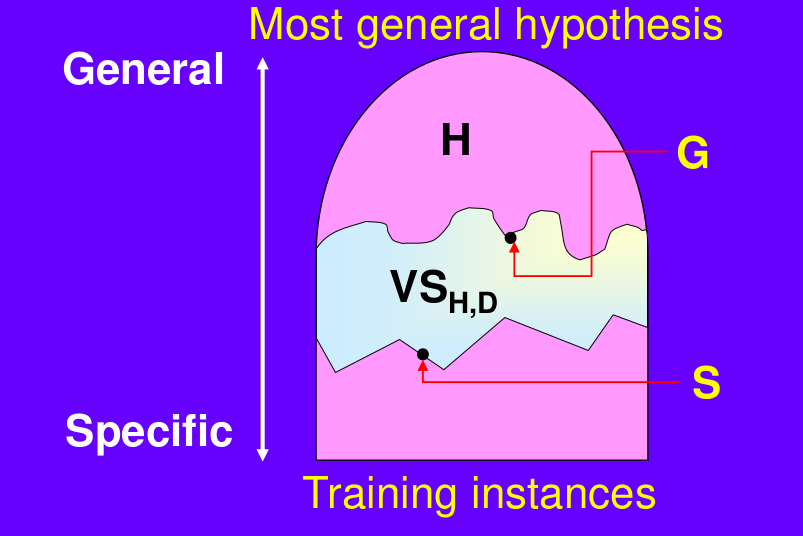
\includegraphics[width=.4\textwidth, height=.3\textheight, keepaspectratio]{compact-representation-vs}}

\end{center}

Il confine generale, o \textbf{general boundary} G, rispetto allo spazio delle ipotesi H e ai dati di addestramento D, è l'insieme dei membri massimamente generali di H consistente con D. $G \equiv \{ g \in H | Consistent(g,D) \land ( \neg \exists g' \in H [(g' >_g g) \land Consistent(g',D)])\}$

Il confine specifico, o \textbf{specific boundary}, S, rispetto allo spazio delle ipotesi H e all'insieme dei dati D, è l'insieme dei membri generali di H consistenti in D. $S \equiv \{ s \in H | Consistent(s,D) \land ( \neg \exists s' \in H [(s >_g s') \land Consistent(s',D)])\}$

Una volta ottenuti questi due insiemi, possiamo definire un algoritmo per eliminare le ipotesi che non sono generali. Questo algoritmo prende il nome di \textbf{Candidate-Elimination}, nel quale in un primo passo si assegna a una variabile G le ipotesi generali in H e in una variabile S si assegnano le ipotesi specifiche in H. Successivamente per ogni esempio di traning d, \textbf{(controllo1)} si controlla se quest'ultimo è un esempio positivo e nel caso si rimuove da G ogni ipotesi inconsistente con d, per poi avviare una funzione UPDATE-S.

La funzione UPDATE-S ha il compito di controllare ogni ipotesi s in S che non è consistente con d, eliminando s da S, per poi aggiungere a S tutte le generalizzazioni minimali h di s tali che h è consistente con d e qualche membro di G è più generale di h. Infine rimuove da S ogni ipotesi che è più generale di un'altra ipotesi in S.

Si ritorna al \textbf{controllo1} e se questo risultasse negativo, si rimuove da S ogni ipotesi inconsistente con d e si avvia una procedura UPDATE-G per aggiornare l'insieme G. Quest'ultima funzione controlla ogni ipotesi g in G che non è consistente con d e in questo caso rimuove g da G, aggiunge a G tutte le specializzazioni minimali h di g tali che h è consistente con d e qualche membro di S è più specifico di h. Infine rimuove da G ogni ipotesi che è meno generale di altre ipotesi in G.

L'algoritmo \textit{candidate-elimination} convergerà verso il target concept a condizione che non ci sono errori negli esempi di training ed è presente qualche ipotesi in HS che descrive correttamente il target concept. Infatti il target concept è appreso quando il confine di S e G converge a un'ipotesi singola e identica.

L'algoritmo genera un un version space vuoto quando l'insieme dei dati di traning contiene errori e il target concept non può essere descritto attraverso ipotesi rappresentative (\textit{hypothesis representation}). Inoltre possiamo dire che l'algoritmo di Candidate-Elimination performa un ricerca bidirezionale, in quanto G e S possono crescere esponenzialmente nel numero di esempi di training.

Quando ci troviamo difronte a concetti appresi parzialmente, abbiamo una minore confidenza nella classificazione in casi ambigui, ma potremmo attuare un approccio basato sul voto maggiore. In questo approccio assumiamo che tutte le ipotesi in H sono uguali a priori, successivamente potremmo decidere in base:

\begin{itemize}
\item al maggior numero di voti, i quali forniscono la classificazione più probabile per la nuova istanza,
\item alla percentuale di ipotesi che votano positivamente, interpretando questo come la probabilità che l'istanza sia positiva dato il dato di training.
\end{itemize}

In questo ci viene in aiuto un algoritmo di \textit{interactive learning} che sceglie la nuova istanza (\textbf{query}) e restituisce la corretta classificazione mediante un oracolo esterno. Se l'algoritmo sceglie sempre una query che è soddisfatta solo da metà delle ipotesi in VS, allora il target concept può essere trovato in $log_2 |VS|$ steps.

Un problema da affrontare in questi tipi di problemi consiste nella gestione del rumore nelle istanze. Per poterlo gestisce si potrebbero rendere più blande le condizioni che descrivono la coerenza dei concetti con tutte le istanze di addestramento. Inoltre se si hanno un numero limitato e predeterminato di esempi classificati in modo errato, si potrebbero mantenere diversi insiemi G e S di consistenza variabile.

\begin{center}

\fbox{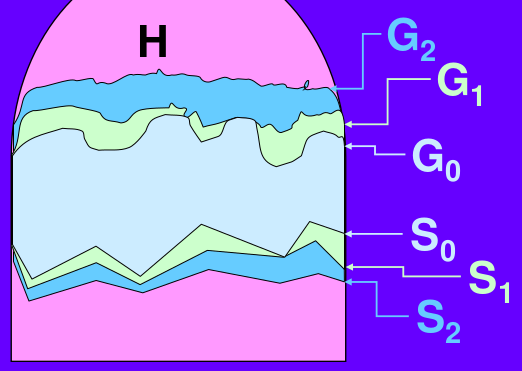
\includegraphics[width=.4\textwidth, height=.3\textheight, keepaspectratio]{compact-representation-error}}

\end{center}

L'insieme $S_i$ è coerente con tutti tranne gli i esempi di allenamento positivi. L'insieme $G_i$ è coerente con tutti tranne gli i esempi di allenamento negativi. Quando $G_0$ incrocia $S_0$ l'algoritmo può concludere che nessun concept nello spazio delle regole è coerente con tutte le istanze di assestamento. L'algoritmo può recuperare e provare a trovare un concetto coerente con tutti gli esempi di addestramento tranne uno.

Una fondamentale proprietà dell'inferenza deduttiva afferma che: "un algoritmo di apprendimento che non crea nessuna assunzione a priori riguardante l'identità del target concept, non ha basi relazionali per qualsiasi istanza invisibile". Questa proprietà prende il nome di \textbf{inductive bias} che può essere definita formalmente come segue.

\textbf{Definizione formale di inductive bias.} Consideriamo:
\begin{itemize}
\item un algoritmo L di concept learning
\item un insieme X di tutte le istanze
\item un target concept c
\item degli esempi di training $D_c = \{ <x,c(x)>\}$
\item denotiamo con $L(x_i,D_c)$ la classificazione assegnata all'istanza $x_i$ da L dopo l'allenamento sui dati $D_c$
\end{itemize}

L'inductive bias di L è qualsiasi insieme minimo di asserzioni B tale che per qualsiasi target concept c e corrispondenti esempi di addestramento $D_c$: $(\forall x_i \in X) [( B \wedge D_c \wedge x_i ) \rightarrow L(x_i,D_c)]$ . Alcuni sistemi induttivi di modellazione possono essere espressi mediante sistemi deduttivi equivalenti. Il cosiddetto inductive bias è un input esplicito begli algoritmi dei sistemi deduttivi.

Analizziamo l'introduzione dell'inductive bias all'interno dell'algoritmo del candidate-elimination. Il target concept c è contenuto nello spazio delle ipotesi H. Da $c \in H$ segue deduttivamente $ c \in  VS_{H,D}$. In questo algoritmo L restituisce la classificazione $L(x_i,D_c)$ se e solo se ogni ipotesi in $VS_{H,D}$ produce anche questa classificazione, includendo anche le ipotesi $c \in VS_{H,D}$ (inductive bias). Quindi $c(x_i)=L(x_i,D_c)$.

Il bias induttivo è un mezzo non procedurale per caratterizzare la politica degli algoritmi di apprendimento per generalizzare oltre i dati osservati. Confrontiamo diversi algoritmi di apprendimento in relazione all'inductive bias. 

Nell'algoritmo \textbf{Rote learning}, si memorizzano gli esempi, viene classificato x se corrisponde a un esempio osservato in precedenza. In questo tipo di algoritmo non c'è nessun inductive bias. Per quanto riguarda l'algoritmo \textbf{candidate elimination}, l'inductive bias consiste nel target concept rappresentato dal suo spazio di ipotesi. Mentre per quanto riguarda l'algoritmo \textbf{Find-S}, l'inductive bias è il target concept rappresentato dal suo spazio di ipotesi e da tutte le istanze negative a meno che il contrario non sia implicato dalla sua altra conoscenza (una sorta di ragionamento predefinito o non monotono). 

Per apprendere concetti disgiunti si può utilizzare l'algoritmo Candidate-Elimination, il quale è un algoritmo con il minimo impegno, che generalizza solo quando è forzato a farlo. Però la disgiunzione fornisce un modo per evitare qualsiasi generalizzazione, per uci l'algoritmo non è mai costretto a farlo. Per apprendere i concetti disgiuntivi, bisogna trovare un metodo per controllare l'introduzione di disgiunzioni, in modo da prevenire disgiunzioni banali. La copertura sequenziale, o \textbf{sequential covering}, è un approccio diffuso all'apprendimento di serie di regole.

Vi sono inoltre particolari algoritmi di copertura sequenziale che performano ripetutamente l'algoritmo di candidate-elimintaion per la ricerca di diverse descrizioni congiuntive che insieme coprono tutte le istanze di training. Ad ogni iterata, si trova un concetto congiuntivo che è coerente con alcuni degli esempi di training positivi e tutti gli esempi di training negativi. I casi positivi che sono stati presi in considerazione vengono rimossi da ulteriori considerazioni e il processo viene ripetuto finché tutti gli esempi positivi non sono stati coperti.

Uno pseudo-codice dell'algoritmo di copertura sequenziale è il seguente:

\textbf{Sequential-Covering(Target-attribute,Attributes,Examples,Threshold)}\\
Learned-rules $\leftarrow \emptyset$\\
Rule $\leftarrow$ LEARN-ONE-RULE (Target-attribute,Attributes,Examples)\\
while PERFORMANCE(Rule, Examples) $>$ Threshold do:\\
$\{$
Learned-rules$\rightarrow$ Learned-rules $\cup \{ Rulle \}$
Examples $\rightarrow$ Examples - $\{$ examples coorrettamente coperti da Rule $\}$
Rule $\rightarrow$ LEARN-ONE-RULE(Target-attribute,Attributes, Examples)
$\}$
Learned-rules $\rightarrow$ sort Learned-rules in accordo con PERFORMANCE over Examples
return Learned-rules


All'interno dell'algoritmo di copertura sequenziale viene utilizzato un particolare algoritmo chiamato \textbf{LEARN-ONE-RULE}. Questo particolare algoritmo accetta un insieme di esempi di traning sia positivi che negativi e restituisce una singola regola che copre tutti gli esempi. Questo algoritmo ha il pregio di essere molto accurato, ma non ha un'alta copertura. Questo algoritmo viene implementato attraverso l'algoritmo Candidate-Elimination. 

Si inizia inizializzando S, il quale conterrà un esempio positivo di training. Per ogni istanza di training negativa si applica la routine Update-G a G. Scegliere una descrizione g da G come una congiunzione per l'insieme delle soluzioni. Poiché Update-G è stato applicato utilizzando tutti gli esempi negativi, g non copre esempi negativi. Tuttavia, g può coprire molti degli esempi positivi. A questo punto si rimuove da ulteriori considerazioni tutti gli esmpi positivi coperti da g. Infine si ripete tutti questi procedimenti fino a quando tutti gli esempi sono coperti.

Un approccio diverso per implementare l'algoritmo LEARN-ONE-RULE è l'\textbf{algoritmo di ricerca General-to-Specific}, mediante il quale si organizza lo spazio di ricerca mediante un ordinamento dal generico allo specifico e si esplora lo spazio attraverso una \textbf{greedy fashion}. Nello specifico si utilizza una ricerca greedy toop-down o general-to-specific. 

La ricerca dello spazio per le precondizioni delle regole iniziando considerando la precondizione della regola più generale possibile. Ad ogni passaggio, viene aggiunto il test che migliora maggiormente le prestazioni della regola. L'aggiunta di un nuovo test restringe la copertura della regola. Il test "migliore" è quello che include il maggior numero possibile di esempi positivi ed esclude il maggior numero possibile di esempi negativi. Supponiamo che una regola copra un totale di t istanze, di cui p sono esempi positivi e t-p sono esempi negativi. Poi scegli la regola che massimizza il rapporto di purezza p/t.

Un esempio di algoritmo separete and conquer è il seguente:

\begin{center}

\fbox{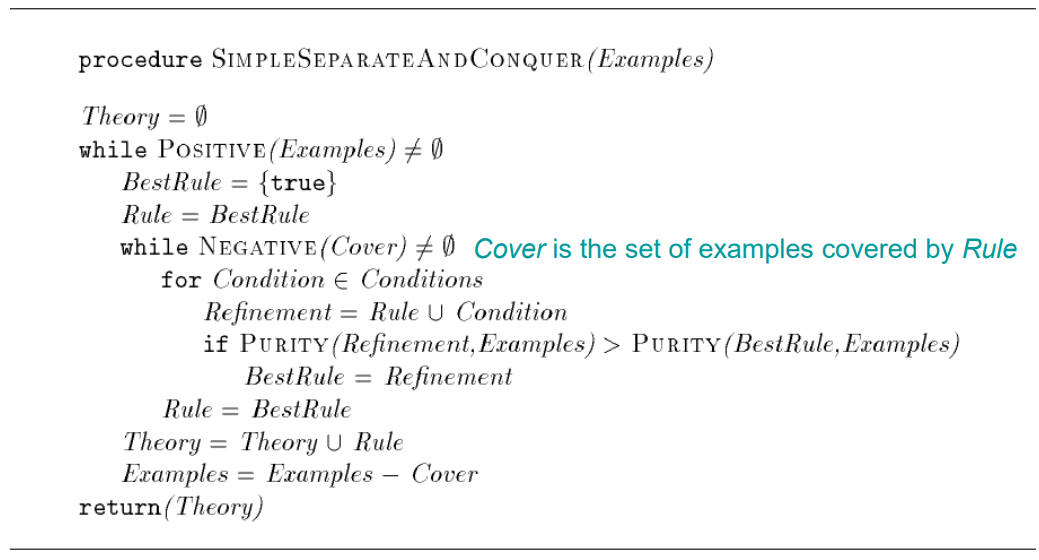
\includegraphics[width=.8\textwidth, height=.5\textheight, keepaspectratio]{seperate-and-conquer-allgoritmo}}

\end{center}

Tutti gli algoritmi di seperate and conquer condividono la struttura base. Mentre, molti task di apprendimento richiedono delle modifiche a questo procedimento. Per esempio, la procedura di overfittin se c'è un po' di noisy all'interno dei dati. Pertanto molti algoritmi allentano questo vincolo e utilizzano criteri di arresto o metodi di post-elaborazione per essere in grado di apprendere teorie più semplici che non sono complete e coerenti, ma sono più predittive su dati invisibili.

Altri algoritmi sostituiscono la ricerca dall'alto verso il basso del whileloop interno con una ricerca dal basso verso l'alto, in cui le regole vengono successivamente generalizzate a partire da una regola più specifica (ad esempio costituita da uno degli esempi positivi stessi). Tuttavia, altri algoritmi non utilizzano hillclimbing, ma impiegano algoritmi di ricerca meno miopi come la beam search o la bestfirst search.

La \textbf{Beam Search} è una ricerca dal generale allo specifico viene implementata come una ricerca greedy depth-first senza backtracking. In questo algoritmo vi è il pericolo di una scelta subottimale in ogni fase. A volte per evitare questo rischio, l'algoritmo viene performato attraverso una lista di k candidati migliori a ogni step e successivamente viene scelto il migliore.

Un altro problema che si incontra nell'algoritmo di separate and conquer è che il tipo delle condizioni usate nella formulazione delle ipotesi. Questo basilare algoritmo può formulare solo regole in logica proposizionale, ma la programmazione logica induttiva ha sviluppato algoritmi che possono imparare le regole nella logica del primo ordine. Un generico algoritmo di apprendimento delle regole separate and conquer che chiama varie subroutine che possono essere utilizzate per istanziare l'algoritmo generico in algoritmi specifici noti dalla letteratura.

\begin{center}

\fbox{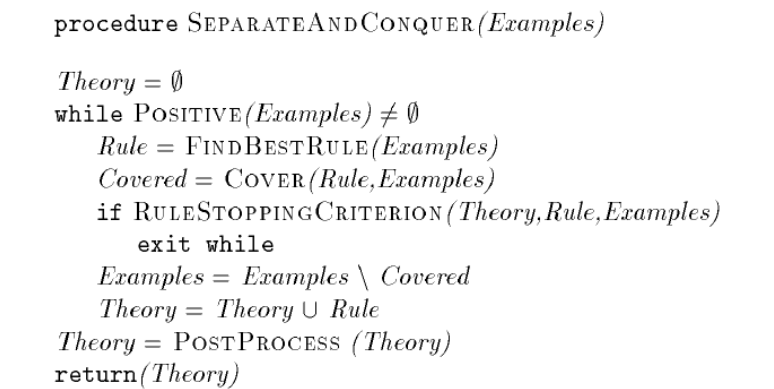
\includegraphics[width=.8\textwidth, height=.5\textheight, keepaspectratio]{seperate-and-conquer-allgoritmo2}}

\end{center}

SeparateAndConquer inizia con una teoria vuota. Se ci sono esempi positivi nel set di addestramento chiama la subroutine FindBestRule per apprendere una regola che coprirà un sottoinsieme degli esempi positivi. Tutti gli esempi coperti vengono quindi separati dal set di addestramento, la regola appresa viene aggiunta alla teoria e un'altra regola viene appresa dagli esempi rimanenti. Le regole vengono apprese in questo modo fino a quando non rimangono esempi positivi o fino a quando RuleStoppingCriterion non viene attivato. Spesso la teoria risultante viene sottoposta a PostProcessing.

\begin{center}

\fbox{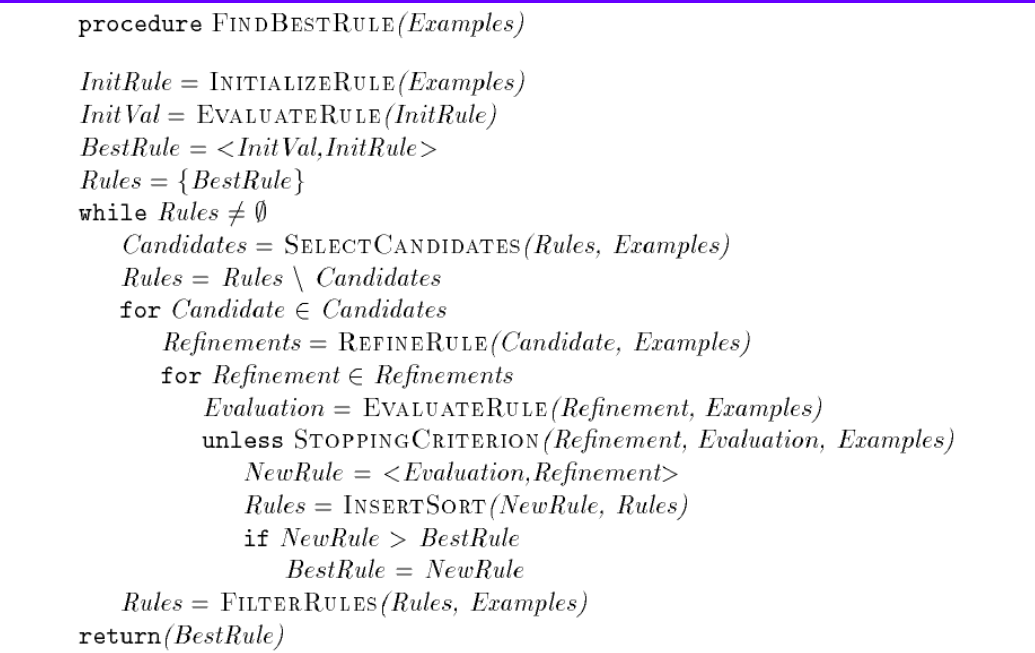
\includegraphics[width=.8\textwidth, height=.5\textheight, keepaspectratio]{seperate-and-conquer-allgoritmo3}}

\end{center}

La procedura FindBestRule cerca nello spazio delle ipotesi una regola che ottimizzi un determinato criterio di qualità definito in EvaluateRule. Il valore di questa funzione euristica di solito è "gli esempi più alti, più positivi e meno negativi sono coperti dalla regola del candidato". FindBestRule gestisce Rules, una lista ordinata di regole candidate, che viene inizializzato dalla procedura InitializeRule. Le nuove regole verranno inserite in punti appropriati (InsertSort), in modo che le regole siano sempre ordinate in ordine decrescente dalle valutazioni euristiche delle regole.

Ad ogni ciclo SelectCandidates seleziona un sottoinsieme di queste regole candidate, che vengono poi raffinate utilizzando RefineRule. Ogni perfezionamento viene valutato e inserito nell'elenco delle regole ordinate a meno che StoppingCriterion non lo impedisca. Se la valutazione di NewRule è migliore della migliore regola trovata in precedenza, BestRule viene impostata su NewRule. FilterRules seleziona il sottoinsieme dell'elenco di regole ordinate che verrà utilizzato in ulteriori iterazioni. Quando tutte le regole candidate sono state elaborate, verrà restituita la regola migliore.

Ad esempio, supponiamo di voler istanziare l'algoritmo generico nel semplice algoritmo separa e conquista. SimpleSeparateAndConquer cerca nello spazio delle ipotesi in modo dall'alto verso il basso. Initialize Rule restituirà quindi la regola più generale, ovvero la regola con il corpo {true}. RefineRule specializzerà una determinata regola aggiungendovi una condizione. Le regole saranno valutate dalla percentuale di esempi coperti che sono positivi, cioè EvaluateRule implementerà la subroutine Purity usata nel semplice algoritmo separate-and-conquer.

FilterRules lascerà passare solo il miglior perfezionamento per l'iterazione successiva, in modo che SelectCandidates abbia sempre una sola scelta. Insieme, queste due procedure implementano la ricerca in salita. A partire dall'elenco ordinato di tutti i perfezionamenti verrà utilizzato solo il primo (e migliore) elemento, questa parte del codice è equivalente alla parte corrispondente in SimpleSeparateAndConquer. Entrambi i criteri di arresto saranno sempre falsi e le regole apprese non verranno postelaborate.

Consideriamo adesso gli algoritmi di simultaneous covering con gli algoritmi di sequential covering. Gli algoritmi di sequential covering sono i più lenti. Per imparare un set di n regole, ogniuna delle quali contiene k attribute-value test nelle loro precondizioni, gli algoritmi di sequentiial covering performeranno $n \times k$ step primitivi di ricerca, indipendentemente dalle scelte.

Gli algoritmi di copertura simultanea sono generalmente veloci, poichè ogni test coon m possibili risultati contribuisce a scegliere le precondizioni per almeno m regole. Gli algoritmi di copertura sequenziale effettuano un gran numero di scelte indipendenti, mentre gli algoritmi di copertura simultanea effettuano un basso numero di scelte dipendenti.

Alcune volte ci si chiede se conviene indurre le regole direttamente o convertire un decision tree in un insieme di regole. La risposta a questa domanda dipende in base a quanti i dati di traning sono disponibili. Se i dati sono abbondanti, possono supportare il maggior numero di decisioni indipendenti richieste dagli algoritmi di copertura sequenziale. Se i dati sono scarsi, la condivisione delle decisioni relative ai presupposti di regole diverse può essere più efficace.

Inoltre bisogna prendere in considerazione anche il task di apprendimento. Se la descrizione del concetto è altamente disgiuntiva con molte condizioni indipendenti, gli algoritmi di apprendimento dell'albero decisionale funzionano male quando i dati sono scarsi.

Nell'apprendimento single-concept, l'elemento appreso è presentato con positive e negative istanze dello stesso concetto. Il sistema deve cercare le regole che descrivono il concetto di studio. Dato u nuovo caso x, se non soddisfa le precondizioni di ogni regola, deve essere considerata come un'istanza negativa. Altrimenti il sistema potrebbe apprendere le regole sia per le istanze positive che per quelle negative del concetto. Quest'ultimo è un caso semplice di multiple-concept learning, nel quale le precondizioni non sono necessariamente mutuamente esclusive.

Quando si classifica un nuovo caso senza il partizionamento dello spazio delle istanze, possiamo ritrovarci in tre casi:

\begin{itemize}
	\item \textbf{nessuna classificazione}: l'istanza non soddisfa nessuna precondizione.
	\item \textbf{singola classificazione}: l'istanza soddisfa le regole di precondizione con la stessa conclusione, sia che essa sia positiva, sia che essa sia negativa.
	\item \textbf{classificazione multipla}: l'istanza soddisfa le regole di precondizione con differenti conclusioni.
\end{itemize}

Nell'apprendimento di concetti multipli, il sistema di apprendimento viene presentato con esempi di formazione che sono istanze di diversi concetti e deve trovare diverse descrizioni di concetti. Per ogni descrizione di concetto, c'è una regione corrispondente nello spazio dell'istanza. Quando i concetti sono indipendenti, un problema di apprendimento con più concetti può essere riformulato come una sequenza di problemi di apprendimento con un singolo concetto.

L'unione degli insiemi di regole apprese per ogni concetto è l'output dell'algoritmo di apprendimento multiple concept. Se i concetti si escludono a vicenda, la classificazione multipla può essere un risultato indesiderato. Per evitare classificazioni multiple, l'aggiunta di una nuova regola all'insieme delle regole apprese può richiedere la modifica delle precondizioni delle regole esistenti (problema di integrazione della conoscenza. Quando i concetti sottostanti si sovrappongono, la classificazione multipla potrebbe essere una caratteristica desiderabile.

Nei problemi di apprendimento di concetti multipli, gli esempi sono tipicamente descritti da vettori di caratteristiche: $<a_1,a_2,\dots,a_n,c>$, dove c è il target attribute. Distinti valori di c rappresentano differenti concetti, i quali sono intesi come mutuamente esclusivi, cioè indipendenti.

Nel caso generale, gli esempi possono essere descritti da vettori di feature: $<a_1,a_2,\dots,a_n,c_1,c_2,\dots,c_m>$ dove $c_i$ sono gli attributi target. I concetti non sono necessariamente indipendenti. Le regole apprese possono includere queste dipendenze concettuali. Lo spazio dell'istanza di un problema di apprendimento a concetto singolo è definito anche da alcuni attributi target. Per decidere quali attributi dovrebbero essere considerati, bisogna scoprire le dipendenze tra gli attributi prima di iniziare il processo di apprendimento, per poi definire gli spazi delle istanze di conseguenza.

Eventuali dipendenze tra attributi possono essere rilevate mediante tecniche statistiche (misura lambda, presentata nella sezione sull'analisi delle associazioni). Le dipendenze concettuali possono essere scoperte online, cioè durante il processo di apprendimento, lavorando simultaneamente con diversi spazi di istanza per ogni problema di apprendimento. Ciò equivale a esplorare diversi spazi di ricerca per ogni concetto da apprendere.

\newpage

\section{K-Means}

Alcuni algoritmi per eseguire il clustering sui dati e trovare tutti i gruppi di istanze simili all'interno dei dataset sono ad esempio il k-means, EM o il Cobweb. I cluster possono essere visualizzati e comparati con i veri cluster, se presenti.

Questo algoritmo prevede la definizione preventiva del numero di cluster, successivamente viene scelto casualmente un insieme di k punti chiamati \textbf{centroidi} che rappresentano i cluster iniziali. Il clustering procede iterativamente nel seguente modo:

\begin{itemize}
\item Assegna ogni punto al cluster il cui centroide è più vicino, generalmente si utlizza la distanza euclidea;
\item Calcola i nuovi centroidi di ogni cluster come la media dei punti che vi appartengono;
\item ripete i passaggi fino a quando non ci sono più cambiamenti significativi nella composizionne dei cluster.
\end{itemize}

Non sempre questo algoritmo identifica un raggruppamento perfetto, infatti il procedimento viene ripetuto scegliendo le distanze iniziali casualmente ed effettuando diversi raggruppamenti da cui scegliere alla fine. Tra i diversi raggruppamenti verrà scelto quello che minimizza le varianze complessivamente, ossia quello che minimizza la total variation within cluster.

Andando ad analizzare i vantaggi e gli svantaggi. Tra i vantaggi possiamo vedere come questo algoritmo sia semplice da implementare con un'efficienza pari a O(nkdi) dove:

\begin{itemize}
\item d è la dimensionalità
\item n è la cardinalità del dataset.
\item k è il numero di cluster da identificare
\item i è il numero di iterazioni necessarie per convergere
\end{itemize}

Mentre tra gli svantaggi possiamo notare che è necessario fissare a priori il numero di cluster k, inoltre questo algoritmo è sensibile al rumore nei dati e alla presenza di outlier, il risultato finale dipende da partizionamento scelto inizialmente. Inoltre i cluster assumono forzatamente forme sferiche, finendo sempre l'iterazione trovando i minimi locali.

Se dovessimo dividere l'algoritmo in diversi step, possiamo definirne 6:
\begin{itemize}
\item \textbf{Step 1}: viene scelto il numero k di cluster in cui selezionare i dati (nel nostro esempio 3)
\item \textbf{Step 2}: vengono selezionate randomicamente 3 istanze che andranno a rappresentare i 3 cluster iniziali.
\item \textbf{Step 3}: viene calcolata la distanza tra il primo punto e i 3 cluster iniziali
\item \textbf{Step 4}: assegna ogni punto al cluster più vicino
\item \textbf{Step 5}: una volta assegnati tutti i punti, viene calcolata la media di ogni cluster.
\item \textbf{Step 6}: si riassegnano le istanze basandosi sulle medie in modo iterativo finchè all'ultima iterazione non si noti variazioni rispetto all'iterazione precedente.
\end{itemize}

Non sempre l'algoritmo K-means identifica un raggruppamento perfetto, infatti inizialmente sceglie le istanze casualmente ed effettua diversi raggruppamenti da cui scegliere alla fine.

Ci sono due metodi principali per scegliere il numero k di cluster. Attraverso il metodo \textbf{elbow method}, nel quale si minimizza la distanza tra i punti di un singolo cluster e si massimizza la distanza tra i cluster. Per calcolare la distanza tra due cluster si utilizza la formula del WCSS, ovvero la somma dei quadrati delle differenze tra i vari punti dei cluster.

Mentre se si decide di scegliere il metodo \textbf{silhouette}, per ogni istanza i calcola la distanza media tra i e ogni altra osservazione j all'interno del cluster in cui i è stata raggruppata. In formula: $a(i) = \dfrac{1}{|C|-1} \sum_{j \in C_I, i \not = j} d(i,j)$. Per ogni istanza i calcola la distanza media tra i e ogni altra osservazione j all’interno degli altri cluster (cluster-wise) diversi da quello in cui risiede i e salva tale media soltanto per il cluster più vicino al cluster di i. Chiama questo valore b(i). In formula: $b(i) = min_{J \not = I} \dfrac{1}{|C_J|} \sum_{j\in C_J} d(i,j)$.

Infine si definisce lo score Silhouette s(i) per i come segue:
\begin{itemize}
\item $1 - \dfrac{a(i)}{b(i)}$ se a(i)$<$b(i)
\item 0 se a(i) $=$ b(i)
\item $\dfrac{b(i)}{a(i)} - 1$ se a(i) $>$ b(i)
\end{itemize}

Inoltre il valore s(i) sarà sempre compreso tra -1 e 1.

Per superare il problema di dover specificare i k cluster, possiamo utilizzare l'algoritmo \textbf{DBSCAN}, il quale è molto robusto in relazione agli outlier. Inoltre questo algoritmo analizza la densità locale alle osservazioni per individuare raggruppamenti anche in forma diversa da quella sferica. Questo è dovuto all'utilizzo del concetto di \textit{core-point} rispetto ad un numero minimo minPts, input utente, di punti vicini ad una determinata istanza e se tale istanza ha in un intorno almeno minPts istanze, allora è considerata core-point.

Dopo aver identificato tutti i core-point, DBSCAN ne prende uno a caso e lo assegna al primo cluster. Quindi assegna allo stesso cluster tutti i core-point nell'intorno del core-point preso casualmente. DBSCAN fa questo per ogni core-point estendendo il cluster finché non raggiunge i punti che non sono core-point.

Per ogni istanza che non è core-point, essa viene inglobata nel cluster se è vicina ad un core-point del cluster appena formato
le istanze che non sono core-point consentono a DBSCAN di fermarsi poiché si è in prossimità di uno spazio delle osservazioni a minore densità rispetto allo spazio denso di core-point.

Stessa cosa viene fatta per altre istanze separate dal primo cluster per identificare il secondo cluster, il terzo e cosi via. Al termine, le istanze che non sono core-point che non appartengono a nessun cluster vengono considerate outlier.

Vi è un altro tipo di cluster è il \textbf{cluster gerarchico}, il cui obiettivo è quello di decomporre gerarchicamente la collezione di individui in una collezione di cluster innestati. Il risultato è rappresentato in forma di dendrogrammi all'interno del quale i nodi rappresentano i possibili cluster., i quali vengono generati bottom-up o top-down.

\newpage

\section{Decision Trees}

Gli alberi di decisione sono usati in task di classificazione, ovvero l'assegnazione di oggetti a categorie che si escludono a vicenda. Il modello predittivo assume la forma di un decision tree, spesso quella specifica del binary tree.

Per costruire un decision tree, in letteratura ci sono diversi metodi tra i quali:
\begin{itemize}
\item Metodi di partizionamento ricorsivi, derivanti dalla disciplina della statistica
\item Induzione di alberi decisionali, derivanti dal Machine Learning
\item Costriuzione di alberi di classificazione, derivanti dal pattern recognition.
\end{itemize}

Un importante decision tree è quello definito come \textbf{C4.5}, che accetta una collezione di casi di training, ognuno dei quali ha una tupla di valori da un insieme di attributi prefissati o \textbf{variabili indipendenti} e una classe attributo o \textbf{variabile dipendente}. Un attributo $A_i$ è descritto come continuo o discreto in base se i suoi valori sono numerici o nominali.

C4.5 utilizza test di due tipi, ognuno dei quali implica un singolo attributo $A_i$. Se quest'ultimo è discreto, i possibili test sono:

\begin{itemize}
\item z risultati, uno per ogni valore di $A_i$
\item $2 \leq w \leq z$ risultati, dove G = $\{ G_1,G_2,...,G_w\}$ è una porzione dei valori di $A_i$.
\end{itemize}

Se $A_i$ è continuo, viene suddiviso in corrispondenza di un valore di soglia derivato. Il test viene diviso nel momento $A_i \leq \theta$ (o a $A_i > \theta$) con risultati vero o falso. In questo caso per determinare quale attributo classifica meglio il dato, si utilizza l'entropia. Prendendo in considerazione:
\begin{itemize}
\item S come l'insieme degli esempi di training analizzati
\item $C_j$ una classe label in $C_1,C_2,...,C_k$.
\item RF($C_i$,S), i=1,...,k le relative frequenze di classi in S che appartengono alla classe $C_i$
\end{itemize}

possiamo considerare l'entropia E su S calcolata come segue: $E(S) = -\sum_{i=1...k} RF(C_i,S)log(RF(C_i,S))$. L'entropia misura il grado di incertezza contenuto in S.

Da notare come questo valore assume il valore massimo quando gli eventi sono equiprobabili. Questa è una buona cosa poiché un insieme di eventi ugualmente probabili è quanto mai incerto. Mentre assume un valore minimo quando solo uno degli eventi ha una probabilità diversa da zero.

Considerando due classi di problemi ($C_1$=positivo, $C_2$=negativo) dove:
\begin{itemize}
\item p è la porzione degli esempi positivi in S,
\item n è la porzione negativa di esempi in S,
\end{itemize}

l'entropia di S è computata come: $E(S) = -p log_2 p - n log_2 n$.

Un altro valore che può essere utilizzato per la selezione dei test è il cosiddetto \textbf{information gain}, che rappresenta la riduzione prevista dell'entropia a causa della distribuzione delle istanze su S in accordo con il test t. Considerando $S_1,...,S_z$ il partizionamento di S attraverso il test t sull'attributo $A_i$, l'information gain può essere ottenuto come: $G(S,t) = E(S) - \sum_i \dfrac{|S_i|}{|S|}E(S_i)$. In questo modo si sceglie il criterio che massimizza G(S,t).

Un problema legato a questo parametro consiste nel favorire test con numerosi risultati. In questo caso l'information gain è massimizzato da un test su un attributo chiave che ogni $S_i$ contiene un solo caso. Una prima soluzione a questo problema consiste nel limitare i decision trees a test binari. Però sono possibili più test sullo stesso attributo. Ciò può portare a alberi decisionali che sono ancora più incomprensibili per gli esperti umani di quanto non avvenga normalmente. Inoltre questa soluzione è computazionalmente espansiva.

Una seconda soluzione tiene conto delle potenziali informazioni dalla partizione stessa, senza considerare la classe, quindi in formula: $P(S,t) = - \sum_i \dfrac{|S_i|}{|S|} log(\dfrac{|S_i|}{|S|})$. La maggior parte possibile delle informazioni fornite determinando il valore di un attributo dovrebbe essere utile ai fini della classificazione o, equivalentemente, il meno possibile dovrebbe essere "sprecato". Perciò scegliamo il test t che massimizza la formula $\dfrac{G(S,t)}{P(S,t)}$, definendo così il \textbf{criterio del gain ratio}.

Per trattare i continuous attributes all'interno dell'algoritmo C4.5 si può definire un nuovo attributo valorizzato con valori discreti per testare l'attributo continuo partizionando il valore continuo in un insieme di intervalli discreti e utilizzando $A_c$ = true se $A<c$. Il valore migliore di c è selezionato usando l'information gain.

Però testare tutti i possibili valori di c è impossibile e non necessario, poichè non ci sarebbe nessuna differenza tra due valori c e c' quando non ci sono esempi di traning che assumono un valore intermedio per l'attributo A. Da questo possiamo estrapolare la seguente procedura:

\begin{itemize}
\item Ordinare gli esempi secondo il loro valore per A
\item Per ogni coppia ordinata $X_i,X_{i+1}$ nella lista ordinata, se le classi di $X_i$ e $X_{i+1}$ sono differenti, utilizzo il punto intermedio tra i loro valori come un candidato soglia.
\item Seleziono il miglior candidato in accordo con l'information gain
\end{itemize}

\subsection{Affrontare i valori mancanti (missing values)}

Se incontriamo valori mancanti di A possiamo intraprendere diverse soluzioni:
\begin{itemize}
\item Off-line: affronto il problema durante lo step di data transformation del processo KDD,
\item On-line: modifica il processo di induzione del decision tree per gestire mancanti.
\end{itemize}

Nell'approccio on-line vi sono diversi problemi. Un primo problema è la valutazione dei test. La selezione di un test su cui partizionare il training set viene effettuata sulla base di criteri euristici quali gain e gain ratio. In questo caso nno possiamo valutare la desiderabilità relativa di due test che utilizzano attributi con valori diversi.

Un secondo problema relativo all'approccio online consiste nel partizionare il training set. Una volta che il test è stato selezionato, i casi di addestramento con valori sconosciuti dell'attributo rilevante non possono essere associati a un particolare risultato del test, e quindi non possono essere assegnati a un particolare sottoinsieme $T_i$.

Un ulteriore problema consiste nel classificare un caso sconosciuto. In questo caso ci si chiede come si deve comportare il decision tree nel caso in cui il sistema ha un valore sconosciuto per l'attributo testato?

Analizziamo nel dettaglio i tre problemi. Nel primo il test non fornisce informazioni circa la classe di appartenenza del caso in cui il valore dell'attributo di test è sconosciuto. Il gain ratio può essere alterato considerando i casi con valori sconosciuti come un gruppo aggiuntivo.

Per il problema del partizionamento del dataset, possiamo utilizzare un approccio probabilistico. Supponiamo di avere il test t con z esiti $v_1,v_2,...,v_z$, che partiziona S i z sotto insiemi $S_1,S_2,...,S_z$, l'idea è quella di associare ogni caso in ogni sotto insieme $S_i$ con un peso rappresentante la probabilità che il caso appartenga al dataset:

\begin{itemize}
\item se il caso ha un esito conosciuto con peso 1
\item altrimenti il peso è la probabilità del risultato $v_i$ in quel punto.
\end{itemize}

Per quanto riguarda il terzo problema, se si incontra un nodo decisionale in cui il valore dell'attributo rilevante è sconosciuto, il sistema esplora tutti i possibili risultati e combina aritmeticamente le classificazioni risultanti. Una classificazione è una distribuzione di classi piuttosto che una singola classe. La classe con la probabilità più alta viene assegnata come classe prevista.

\subsection{Svantaggi}

La tecnica di induzione del decision tree è molto efficiente in termini di tempo di elaborazione e fornisce un metodo molto intuitivo per analizzare i risultati. Questa intuitività, soprattutto se confrontata con l'output meno accessibile delle reti neurali, spiega perché gli alberi decisionali sono ancora attraenti. Nonostante tutto hanno degli svantaggi.

Gli attuali metodi di induzione dell'albero decisionale non sono ottimali. Durante la formazione di un albero decisionale, una volta che l'algoritmo prende una decisione sulla base su cui dividere il nodo, tale decisione non viene mai rivista. I metodi per la costruzione di un albero decisionale ottimo hanno una complessità esponenziale.

Gli alberi decisionali soffrono di un problema di errori che si propagano in un albero, un problema molto serio con l'aumentare del numero di classi. Poichè i regression tree funzionano in base a una serie di decisioni locali, se una di queste è sbagliata ogni decisione da quel punto in poi potrebbe essere sbagliata, inoltre non avremmo mai un percorso corretto.

Gli alberi decisionali sono limitati ai problemi che possono essere risolti dividendo lo spazio della soluzione in rettangoli successivamente più piccoli.


In generale, gli alberi decisionali soffrono di frammentazione. Quando l'albero ha molti strati di nodi, la quantità di dati che passa attraverso le foglie inferiori è così piccola che è difficile prendere una decisione precisa sulla classe associata a ciascuna foglia. Per ridurre al minimo la frammentazione, l'analista può potare o tagliare alcune delle foglie e dei nodi inferiori per far collassare efficacemente parte dell'albero. Il risultato è un modello migliorato in cui vengono rivelati i modelli reali piuttosto che il rumore (evitamento dell'overfitting) ed è più semplice da capire.

Generalmente si sceglie ipotesi brevi rispetto a ipotesi lunghe, per svariati motivi. Definiamo H come uno spazio di ipotesi, considerando un errore  nell'ipotesi $h \in H$ questo si ripercuote sui:
\begin{itemize}
\item Training data, e per calcolare l'errore si può definire la funzione $error_{training}(h)$
\item sull'intera distribuzione D di dati, il cui errore si può calcolare definendo la funzione $error_D(h)$.
\end{itemize} 

L'ipotesi $h \in H$ overfitta i dati di traning se c'è un ipotesi alternativa $h' \in H$ tale che $error_{training}(h)<error_{traning}(h')$ e se $error_D(h)>error_D(h')$ Si dice che un'ipotesi, h, superi l'insieme di addestramento, D, quando esiste un'ipotesi, h', che supera h sulla distribuzione totale delle istanze in cui D è un sottoinsieme.

Questo può accadere se c'è rumore all'interno dei dati che crea un albero grande per l'ipotesi h e l'ipotesi h' non fitta. Inoltre avere un numero limitato di campioni, rende le coincidenze sempre più possibili, anche se gli attributi non correlati all'attributo di destinazione possono partizionare bene i dati di addestramento.

Per evitare l'overfitting possiamo \textbf{fermare la crescita dell'albero} quando lo split dei dati non è statisticamente significante, in quanto non ci sono abbastanza dati per rendere le decisioni  affidabili. Inoltrre per evitare una crescita esponenziale, si potrebbe togliere dall'albero tutti quei nodi per i quali non si hanno sufficienti evidenze.

\subsection{Training set vs. Validation set}

A volte i dati sono partizionati in training set e testing set. I primi vengono utilizzati pera apprendere, mentre i secondi per validare. Tipicamente si utilizza una proporzione del 70-30%

\subsection{Metodi di selezione dei cicli}

\subsubsection{Reduced error pruning (REP)}

In questo caso si utilizza un set di potatura per stimare l'accuratezza dei sottoalberi e l\' accuratezza sui singoli nodi. Considerando un sub-tree con un nodo v come vertice, si definisce il \textbf{Gain della potatua a v} $= $ \# classificazioni errate in T - \# classificazioni errate in v. Si pota T al nodo v solo se il gain è positivo. In questo caso bisogna rispettare una \textit{restrizione Bottom-up}: T può essere eliminato solo se non contiene un sottoalbero con errore inferiore a T.

\subsubsection{Minimal Error Pruning (MEP)}

Questo algoritmo prende in considerazione per potare i rami se l'errore statistico è minore o uguale all'errore di backed-up, e l'errore del sotto albero di .

\begin{equation*}
E(T) = min(e(v), \sum\limits_{i} p_iE(T_i))
\end{equation*}

Per stimare l'errore e(v) si usa Laplace o la stima m di probabilità.

La \textbf{stima di Laplace} al nodo v, con N esempi, con $n_c$ il numero di esempi della classe di maggioranza e con k il numero di classi, si ha:

\begin{equation*}
p_c = \dfrac{n_c+1}{N+k}
\end{equation*}

Questa formula assume che tutte le classi hanno la stessa probabilità e il grado di potatura dipende dal numero di classi.

Per risolvere questi problemi si utilizza la stima m, che prende in considerazione $p_{ca}$ ovvero la probabilità della classe C e m, un parametro non negativo.

\begin{equation*}
p_C = \dfrac{p_{Ca}\times m + n_C}{N+m}
\end{equation*}
Questo metodo da importanza agli account con probabilità priori, non risente del numero delle classi, si può variare il valore di m ottenendo una serie di alberi potati differenti. La scelta di m dipende dalla confidenza con i dati

\subsubsection{Pessimistic Error Pruning (PEP)}

Questo algoritmo non richiede un set di potatura per la stima dell'errore, la quale avviene sui nuovi dati direttamente dall'insieme di crescita. Si effettua una stima sulla frequenza relativa con una correzione, considerando la probabilità d'errore.

\begin{equation*}
 q = \dfrac{N-n_c+0.5}{N}
\end{equation*}

dove N rappresenta il numero di esempi e $n_c$ il numero di esempi nella classe maggiore. Inoltre si può calcolare l'errore di un nodo se potato:

\begin{equation*}
q(v) = \dfrac{N_v - n_{C,v} +0.5}{N_v}
\end{equation*}

Mentre l'errore di un sotto albero può essere calcolato come:
\begin{equation*}
q(T) = \dfrac{\sum\limits_{l \in leaf(T)} N_l - N_{C,l} + 0.5}{\sum\limits_{l \in leaf(T)} N_l} 
\end{equation*}

\subsubsection{Error-Based Pruning (EBP)}

In questo caso si decide di potare un sotto albero T se $q(v) \leq q(T) + SE(q(T))$, dove SE è l'errore standard di una statistica X sopra un numero di esempi n:
\begin{equation*}
SE(X) = \sqrt{\dfrac{X(1-X)}{n}}
\end{equation*}

\section{Naive Bayes Classidier - Classificatore Bayesiano}

Il \textbf{Bayesian Framework} è composto da un insieme di dati osservati D ai quali siamo interessati nel determinare le migliori ipotesi da qualche spazio H. Per un task di classificazione, le ipotesi è un classificatore. Il \textit{teorema di Bayes} è un metodo per calcolare la probabilità di un ipotesi basata sulle probabilità a priori e sui dati osservati.

Definiamo:
\begin{itemize}
\item con \textbf{h} le ipotesi

\item con \textbf{P(h)} la probabilità a priori di h, cioè, la probabilità iniziale che valga l'ipotesi h, prima di aver osservato i dati di addestramento. Riflette alcune conoscenze di base che abbiamo sulla possibilità che h sia un'ipotesi corretta.

\item con \textbf{P(D)} la probabilità a priori di D, cioè, la probabilità che i dati di addestramento D vengano osservati non sapendo quale ipotesi sia valida.

\item con \textbf{P(D$|$h)} denotala probabilità di osservare i dati D dato un mondo in cui vale l'ipotesi h.

\item con \textbf{P(h$|$D)} probabilità a posteriori di h, ovvero la probabilità che h sia valida dopo aver visto i dati di addestramento D.
\end{itemize}

Nella formula:
\begin{equation*}
P(h|D) = \dfrac{P(D|h)P(h)}{P(D)}
\end{equation*}

\begin{itemize}
\item $P(h|D)$ cresce con P(h) e con $P(D|h)$
\item $P(h|D)$ diminuisce all'aumentare di P(D), perché quanto più è probabile che D venga osservato indipendentemente da h, tanto meno prove D fornisce a sostegno di h.
\end{itemize}

L'ipotesi $h\in H$ con la massima probabilità è l'ipotesi con \textbf{massimo a posteriori (MAP)}, ovvero:
\begin{equation*}
h_{MAP} = arg  max_{h \in H} P (h|D) = arg  max_{h \in H} \dfrac{P(D|h)P(h)}{P(D)}
\end{equation*} 

Il termine P(D) può essere eliminato dalla formula perchè è una costante indipendente di h. Assumendo che tutte le ipotesi sono altrettanto probabili, le equazioni possono essere ulteriormente semplificate. L'ipotesi che massimizza $P(D|h)$ è le più probabile. $P((D|h)$ è chiamata la probabilità dei dati D data h. Questa ipotesi è chiamata ipotesi di probabilità massima (ML), ovvero:
\begin{center}
$h_{ML} = arg max_{h \in H} P(D|h)$
\end{center} 

A differenza di una ipotesi ML, una ipotesi MAP incorpora la conoscenza a priori.

Per applicare il teorema di Bayes ai problemi di classificazione, definiamo:
\begin{itemize}
\item uno spazio di istanze X
\item $c: X \rightarrow \{0,1\}$, una funzione di classificazione che deve essere appresa
\item uno spazio delle ipotesi H
\item una funzione booleana definita su X tale che $h \in H$: $h : X \rightarrow \{0,1\}$
\end{itemize}

L'obiettivo è di trovare h tale che h(x)=c(x) per tutte le istanze x $\in$ X. L'informazione disponibile è una sequenza di esempi di training $<<x_1,d_1>\dots <x_m,d_m>>$, dove $x_i$ è un'istanza di X e $d_i$ è il valore targe di $x_i$, ovvero $d_i = c(x_i)$.

Se si volesse implementare un \textbf{algoritmo di apprendimento MAP per forza bruta}, basterebbe calcolare per ogni $h \in H$ la probabilità a posteriori:
\begin{equation*}
P(h|D) = \dfrac{P(D|h)P(h)}{P(D)}
\end{equation*} 

L'output dell'ipotesi $h_{MAP}$ con la più alta probabilità a posteriori:
\begin{equation*}
h_{MAP} = arg max_{h \in H} P(h|D)
\end{equation*}

In questo algoritmo si assume che l'insieme dei dati di training D è senza rumore, ovvero $d_i = c(x_i)$. Il concetto target c è contenuto nello spazio dell'ipotesi H. Inoltre si presume che non abbiamo nessuna ragione a priori di credere che un'ipotesi è più probabile di un'altra.

Per stimare P(h), si assume che $P(h_i)$ è uguale per ogni $h_i \in H$, inoltre si assume che la somma di $P(h_i)$ è uguale a uno. Perciò $P(h) = \dfrac{1}{|H|}$ per tutte $h\in H$.

Per stimare $P(D|H)$ si assume:

\begin{equation*}
	P(D|h) = 
	\begin{cases}
		1 \text{ if }  d_i = h(x_i) \; \forall x_i \in D \\
		0 \text{ otherwise}
	\end{cases}
\end{equation*}

La probabilità dei dati D, data l'ipotesi h, è 1 se D è consistente con h, 0 altrimenti.

Per stimare P(D) basta utilizzare il teorema della probabilità e la mutua esclusione delle ipotesi.

\begin{equation*}
P(D) = \sum\limits_{h_i \in H} P(D|h_i)P(h_i) = \sum\limits_{h_i \in VS_{H,D}} 1 \times \dfrac{1}{|H|}+ \sum \limits_{h_i \not \in VS_{H,D}} 0\times \dfrac{1}{|H|} = \dfrac{|VS_{H,D}}{|H|}
\end{equation*}

dove $VS_{H,D}$ è un sotto insieme di ipotesi da H che sono consistenti in D.

Perciò quando h è inconsistente con l'insieme dei dati D, $P(h|D) = 0 \times \dfrac{P(h)}{P(D)} = 0$, altrimenti:

\begin{equation*}
P(h|D) = \dfrac{1 \times \dfrac{1}{|H|}}{\dfrac{|VS_{H,D}|}{|H|}}
\end{equation*}

Sotto le scelte di P(h) e $P(D|h)$, ogni ipotesi consistente ha una probabilità a posteriori di $\dfrac{1}{|VS_{H,D}}$ e ogni ipotesi inconsistente ha una probabilità a posteriori di 0. Perciò possiamo assumere che \textit{ogni ipotesi consistente è un'ipotesi MAP.}

Una classe di leaners consistenti è una classe di algoritmi di apprendimento che produce un ipotesi che commette zero errori sugli esempi di training. Ogni leaner consistente produce un ipotesii MAP, se assumiamo una distribuzione di probabilità uniforme a priori su H e assumiamo che questa sia deterministica, su un insieme di dati di training senza rumore.

Il framework bayesiano consente un modo per caratterizzare il comportamento degli algoritmi di apprendimento (ad esempio, FIND-S), anche quando l'algoritmo di apprendimento non manipola esplicitamente le probabilità. Questa caratterizzazione degli algoritmi di apprendimento è simile nello spirito alla caratterizzazione del pregiudizio induttivo del learner. Invece di modellare il metodo di inferenza induttiva con un sistema deduttivo equivalente, lo modelliamo con un sistema di ragionamento probabilistico equivalente basato sul teorema di Bayes.

\begin{center}

\fbox{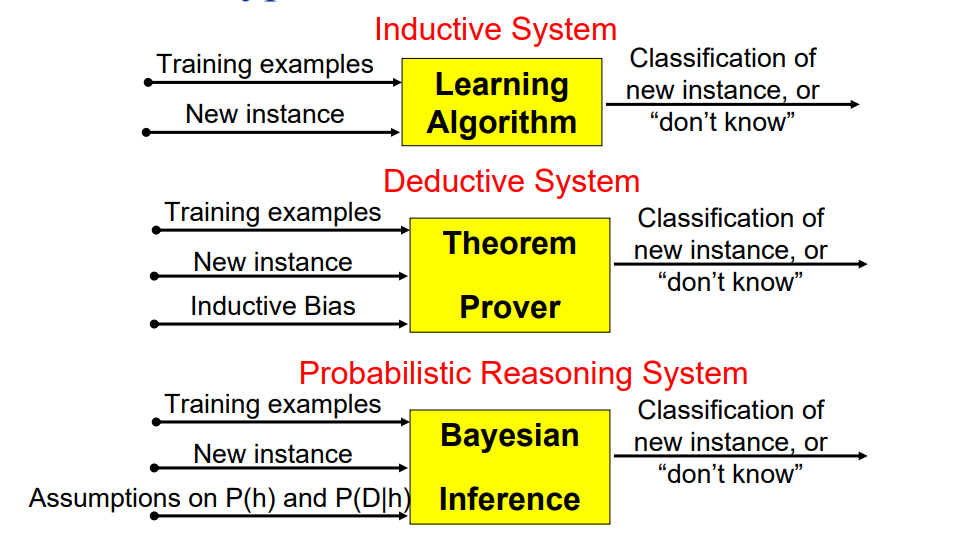
\includegraphics[width=.8\textwidth, height=.5\textheight, keepaspectratio]{different-probabilistic-method}}
\end{center}

Riconsideriamo la definizione di $h_{MAP}$: $h_{MAP} = argmax_{h\in H} P(D|h)P(h)$, potremmo riscriverla cercando di massimizzarla/minimizzarla in termini di $\log_2$:

\begin{equation*}
\begin{split}
h_{MAP} = argmax_{h \in H}(\log_2(P(D|h) + \log_2(P(h))) \\
h_{MAP} = argmin_{h \in H}(- \log_2(P(D|h) - \log_2(P(h)))
\end{split}
\end{equation*}

Nella teoria dell'informazione vi è un problema per decodificare un algoritmo per trasmetter messaggi estratti a caso. La probabilità del messaggio i è $p_i$. Qual è il codice che minimizza il numero previsto di bit che dobbiamo trasmettere per codificare un messaggio estratto a caso? Ci viene in aiuto il teorema di Shannon, il cui codice ottimale assegna $-\log_2(p_i)$ bits per codificare il messaggio i. La lunghezza del messaggio aspettato è: $\sum\limits_i -p_i \log_2 p_i$ 

La lunghezza della descrizione del messaggio i rispetto al codice C, $L_C (i)$, è il numero di bits richiesto per codificare il messaggio i usando il codice C.

In formule:
\begin{equation*}
h_{MAP} = argmin_{h \in H} (- \log_2 P(D|h) - \log_2 P(h))
\end{equation*} 

Che possiamo interpretare alla luce del teorema dii Shannon come:
\begin{itemize}
\item $-\log_2 P(h)$ è la descrizione della lunghezza di h sotto la condizione ottimale per l'ipotesi di spazio H. $\rightarrow L_{C_H}(h) = - \log_2P(h)$ dove $C_H$ è il codice ottimale per lo spazio dell'ipotesi H.
\item  $-\log_2 P(D|h)$ è la lunghezza della descrizione di D data h sotto la sua codifica ottimale $\rightarrow L_{C_{D|h}} = - \log_2 P(D|h)$ dove $C_{D|h}$ è il codice ottimale per descrivere i dati D assumendo che sia chi li via sia il ricevente conoscono l'ipotesi h.
\end{itemize}

Perciò l'ipotesi $h_MAP$ è l'ipotesi h che minimizza la somma: $h_{MAP} = argmin_{h \in H} (L_{C_H}(h) + L_{C_{D|h}}(D|h))$

Il \textbf{principio della lunghezza minima della descrizione } raccomanda di scegliere l'ipotesi che minimizza la somma delle due lunghezze relative alle descrizioni, una che rappresenta l'ipotesi e l'altra che rappresenta i dati data l'ipotesi: $h_{MDL} = argmin_{h \in H} L_{C_1}(h) + L_{C_2} (D|h)$. 

$L_{C_2}(D|h)$ è zero quando l'ipotesi non sbaglia a classificare i dati di traning. Il principio MDL è un bias induttivo che consiglia, analogamente al rasoio di Occam, di scegliere l’ipotesi più semplice (più breve) che spieghi i dati di addestramento. Fornisce un modo per bilanciare la complessità dell'ipotesi con il numero di errori commessi dall'ipotesi. Potrebbe selezionare un'ipotesi più breve che commette alcuni errori rispetto a un'ipotesi più lunga che classifica perfettamente i dati di addestramento. Fornisce un modo per gestire il sovradattamento.

Se confrontassimo 
\begin{equation*}
h_{MDL} = argmin_{h\in H} L_{C_1} (h) + L_{C_2}(D|h)
\end{equation*}
con
\begin{equation*}
h_{MAP} = argmin_{h\in H} L_{C_H} (h) + L_{C_{D|h}}(D|h)
\end{equation*}

risulta chiaro che le ipotesi MAP e il principio MDL sono strettamente collegati. Quando $C_1 = C_H$ e $C_2=C{D|h}$ allora $h_{MDL} = h_{MAP}$.

Invece per garantire che $C_1=C_H$ e $C_2=C_{D|h}$ dobbiamo conoscere tutte le probabilità a priori P(h) come anche tutte le $P(D|h)$. In pratica a volte è più semplice specificare una rappresentazione che cattura la conoscenza sulle probabilità relative delle ipotesi piuttosto che specificare completamente la probabilità di ciascuna ipotesi. Tipicamente, le applicazioni dell’MDL a problemi pratici di apprendimento spesso includono argomenti che forniscono una qualche forma di giustificazione per le codifiche scelte per $C_1$ e $C_2$.

In generale, il classificatore più probabile per una nuova istanza è ottenuta combinando le predizioni delle ipotesi, pesate attraverso le loro probabilità a posteriori. Se l'eventuale classificazione del nuovo esempio può assumere qualsiasi valore $v_j$ dall'insieme V, allora la probabilità $P(v_j|D)$  che la classificazione corretta per la nuova istanza è $v_j$ è solo:

\begin{equation*}
P(v_j|D) = \sum\limits_{h_i \in H} P(v_j | h_i) P(h_i|D) 
\end{equation*}

Qualsiasi sistema che classifica nuove istanze in questo modo è chiamato classificatore ottimale di Bayes o studente ottimale di Bayes. Nessun altro metodo di classificazione che utilizza lo stesso spazio di ipotesi e la stessa conoscenza preliminare può in media superare questo metodo.

\end{document}




